\chapter{Generaci\'on de expresiones referenciales}
\label{sec:seleccion}

Este cap\'itulo est\'a dividido en 4 secciones. En la Secci\'on \ref{generacion-humana} damos definiciones b\'asicas que nos servir\'an a 
lo largo de la tesis. Explicamos los diferentes tipos de expresiones referenciales. Las ERs se diferencian seg\'un el tipo de propiedades que 
contengan, pueden contener propiedades at\'omicas, o relaciones con otros objetos, o ambas. Las ERs tambi\'en se diferencian por la cantidad 
de informaci\'on que contienen. Las ERs \textbf{minimales} contienen s\'olo la informaci\'on indispensable para identificar al target. Las \textbf{sobreespecificadas} contienen m\'as informaci\'on de la m\'inima necesaria para identificar al target, y las \textbf{subespecificadas}, no identifican al target correctamente, sino a un conjunto m\'as grande el cual contiene al target y a otros elementos, porque la informaci\'on que contienen no es suficiente para identificar al target. Las ERs \textbf{plurales}, son expresiones que identifican a un conjunto target que tiene m\'as de un elemento, y las \textbf{parciales}, son las que siendo plurales, no alcanzan a identificar a todos los elementos del conjunto target. Luego explicamos c\'omo los humanos usamos el lenguaje para trasmitir intenciones, y c\'omo esas intenciones son interpretadas por los oyentes, comentamos a cerca de la teor\'ia de \cite{Clark-Marshall81,clark1992arenas} y damos ejemplos que la contradicen, nombramos el rol de la sobreespecificaci\'on y damos ejemplos de uso. Finalmente en la secci\'on, introducimos corpus de ERs existentes: el TUNA, el GRE3D3/7, Stars/2 y el ZOOM.

Luego, en la Secci\'on \ref{sec:tipos_algoritmos} damos los tipos de algoritmos los cuales casi todos tienen una correlaci\'on directa con los tipos de ERs, y justamente dependen de los tipos de ERs que pueden generar, \textbf{determin\'isticos} son aquellos que dado un input fijo, siempre dan la misma ER, \textbf{no-determin\'isticos} son los que pueden dar distintas ER en 2 corridas del algoritmo con el mismo input, que generan \textbf{sobreespecificaci\'on}, que son los que pueden dar ER con m\'as de la m\'inima cantidad de informaci\'on que se necesita para identificar al target, \textbf{plurales}, son los que pueden dar ER para conjuntos de objetos, \textbf{s\'olo singulares}, son los que dan resultado s\'olo para un target singleton, \textbf{relacionales} o \textbf{proposicionales}, cuando pueden o no incluir relaciones y expresiones de los objetos relacionados. Adem\'as contamos la historia del \'area, y explicaremos los algoritmos m\'as conocidos como el incremental, GRAPH, relacional entre otros. 

En la Secci\'on \ref{sec:metricas_evaluacion} damos una introducci\'on a las m\'etricas de evaluaci\'on en el \'area algunas que usan corpus para comparar salidas de algoritmos con ERs dadas por personas, algunas que necesitan jueces humanos y otras que son autom\'aticas. 

Y para finalizar en la Secci\'on \ref{sec:linkeo2} daremos el resumen del cap\'itulo y como se linkea con los dem\'as cap\'itulos.


\section{Generaci\'on \emph{humana} de expresiones referenciales}
\label{generacion-humana}

Esta secci\'on est\'a dividida en 3 partes, en la primer parte veremos los diferentes tipos de ERs. En la segunda parte veremos las premisas en las que se basa la teor\'ia de \cite{Clark-Marshall81}, \cite{clark1992arenas}, y c\'omo algunos experimentos la contradicen. Veremos que la sobreespecificaci\'on es algo com\'un en la mayor\'ia de los contextos, que no est\'a mal visto por parte de los oyentes y que de hecho puede ser \'util en diversos dominios. En la tercer parte presentamos corpora de ERs existentes en el \'area y mostraremos una comparaci\'on entre ellos.
%Los trabajos em\'iricos realizados en el \'area en la Secci\'on \ref{sec:trab_emp} explicaremos como trabaj\'o la gente usando corpora y las m\'etricas de evaluaci\'on en la Seccion \ref{sec:metricas_evaluacion} daremos una introducci\'on a los diferentes tipos de m\'etricas, autom\'aticas, manuales. 

 %(ver si los divido por secciones a los algoritmos...)
%ERORDENAR ESTO
%\cite{arec2:2008:Areces}~mostraron que el algoritmo de refinamiento utilizando el lenguaje de descripci\'on \el como lenguaje formal es capaz de generar 67\% de
%las ERs relacionales en el corpus ~\cite{viethen06:_algor_for_gener_refer_expres} cuando se consideran todos los posibles \'ordenes de las relaciones en el dominio. Esto est\'a en marcado contraste con el an\'alisis hecho en~\cite{viethen06:_algor_for_gener_refer_expres} sobre el cabinet corpus, de algoritmos basados en la propuesta original Dale y de Reiter.
%Los resultados de cobertura reportados sobre Viethen and 
%Dale's sobre el Cabinet corpus significan que~\emph{alg\'un orden} produce una razonablemente amplia cobertura. En otras palabras, se ha demostrado que los algoritmos de refinamiento tienen la capacidad de producir ERs similares a los producidos por los humanos, proporcionado una ordenaci\'on adecuada sobre las relaciones que aparecen
%en la escena de entrada, pero no est\'a claro cu\'al de todos los \'ordenes posibles se debe utilizar. En esta tesis abordamos directamente esta cuesti\'on.

%\section{Clasificaciones b\'asicas de ER y algoritmos GER}

%Esta secci\'on explicaremos los diferentes {\it tipos de ER}, as\'i como los diferentes {\it tipos de algoritmos} para generar algunos de los tipos de ER nombrados.

\subsection{?`Qu\'e tipos de expresiones referenciales existen?}
\label{sec:tipos_er}

Recordemos que una {\bf expresi\'on referencial} (ER), es un sintagma nominal que identifica a un target un\'ivocamente en un contexto dado para un interlocutor particular.

En una ER, una \textbf{propiedad} es una caracter\'istica propia de un objeto. Por ejemplo, en la Figura \ref{GRE3D7-stimulus}, el objeto se\~nalado con la flecha tiene la propiedad {\it forma} con valor {\it esfera}.\footnote{Por simplicidad, en el resto de la tesis vamos a decir ``tiene propiedad {\it esfera}'', cuando queremos decir que el objeto tiene la propiedad forma con valor esfera.} Una \textbf{relaci\'on} caracteriza a un objeto describiendo caracter\'isticas de otro u otros objetos. Por ejemplo, en la Figura \ref{GRE3D7-stimulus}, {\it La pelota que est\'a al lado del cubo grande}, la relaci\'on 'al lado de' necesita describir propiedades de otro objeto, en este caso el {\it cubo grande}.

%Cuando la ER no es relacional solo contiene propiedades del objeto mismo. Ej.: color, tama\~no. Note que quiz\'as el tama\~no sea con respecto a los dem\'as objetos ``la m\'as peque\~na'', pero al no incluir una descripci\'on de otro objeto no la llamamos relacional.\\

De acuerdo a las propiedades o relaciones que una ER incluya, se clasifica en distintos tipos: relacional o no relacional (tambi\'en llamada proposicional), minimal, sobreespecificada, subespecificada o parcial, plural o singular. A continuaci\'on describimos cada uno de estos tipos.
% en cuyo caso es una expresi\'on que no es referencial, la incluimos en nuestras propiedades porque nos va a ser \'util la definici\'on en el Cap\'itulo \ref{sec:corpus}.\\
\begin{itemize}
\item Una ER {\bf proposicional} o no relacional, incluye s\'olo propiedades intr\'insecas del objeto target. Por ejemplo, en la Figura \ref{GRE3D7-stimulus}: {\it La esfera roja}. Las caracter\'isticas de ser esfera y ser roja son propias del objeto identificado y no de su entorno.

\item Una ER es {\bf relacional}, cuando contiene relaciones con otros objetos. En este caso la ER incluye descripciones de los otros objetos. Por ejemplo, en la Figura \ref{GRE3D7-stimulus}: {\it La esfera que est\'a a la derecha del cubo}. {\it A la derecha de} lexicaliza una relaci\'on que necesita describir otro objeto adem\'as del target, en este caso un {\it cubo}.

\begin{figure}[H]
\begin{subfigure}{.5\textwidth}
\centering
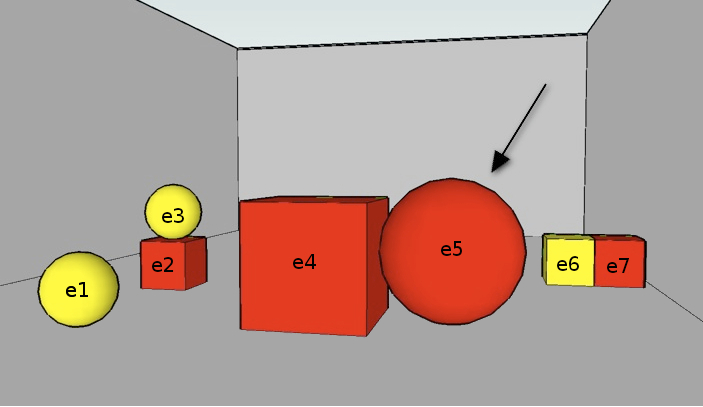
\includegraphics[width=\textwidth]{images/22.jpg}\\[0pt]
\caption{}
\label{GRE3D7-stimulus}
\vspace*{.1cm}
\end{subfigure}
\hspace*{0cm}
\begin{subfigure}{.5\textwidth}
\centering
%\vspace*{-2cm}
\begin{tabular}{l}
 {\it La esfera grande}\\
 {\it La esfera roja que est\'a al lado del cubo rojo} \\
 {\it El objeto que est\'a al lado del cubo grande}\\
 {\it La bola roja}\\
 {\it La pelota a la izquierda del cubo amarillo}\\
 {\it La bola grande}\\
 {\it La esfera que est\'a a la derecha del cubo rojo y a }\\
 {\it la izquierda del cubo amarillo}\\
 {\it La cosa que est\'a a la derecha del cubo del medio}\\
 {\it ...}
 \end{tabular}
\caption{}
\label{GRE3D7-stimulus-er}
\end{subfigure}
\caption{ER para la imagen de la Figura \protect\ref{GRE3D7-stimulus}, y el contexto con objetos identificados.}

\end{figure}


\item \label{sec:minimales} Se dice que una ER es {\bf minimal}, cuando incluye la m\'inima cantidad de propiedades y/o relaciones con otros objetos, con las cuales el target puede ser distinguido en el contexto dado. Notar que puede haber muchas expresiones minimales. Por ejemplo, en la Figura \ref{GRE3D7-stimulus}: {\it La esfera roja} es una ER minimal, como as\'i tambi\'en lo es {\it La esfera grande}, o {\it La esfera a la derecha del cubo}. Para verificar que estas ERs son minimales, intentemos sacar alguna propiedad, si de {\it La esfera roja} sacamos esfera, ya no podemos identificar al target, si sacamos roja, tampoco. Lo mismo pasa para {\it La esfera grande}. Veamos que pasa con {\it La esfera a la derecha del cubo}, si sacamos {\it esfera} tenemos otro objeto adem\'as del target que tambi\'en tiene a la izquierda un cubo. Si sacamos {\it a la derecha de} tampoco identifica al target. 

\item Cuando la ER contiene m\'as informaci\'on de la m\'inima necesaria para distinguirlo de los dem\'as objetos en el contexto dado, se dice que la ER es {\bf sobreespecificada}. Por ejemplo: {\it La esfera roja grande} en la Figura \ref{GRE3D7-stimulus} es sobreespecificada porque se le puede sacar {\it grande} y sigue siendo una ER correcta, o se le puede sacar {\it roja} y tambi\'en lo sigue siendo. \label{er-sobreespecificadas}

\item Una expresi\'on\footnote{Estrictamente hablando, una expresi\'on subespecificada no es una ER dado que no identifica un\'ivocamente al target, sin embargo, en esta tesis hablaremos en ocasiones de ERs subespecificadas para referirnos a \'estas expresiones que no alcanzan a ser referenciales.} es {\bf subespecificada} cuando no puede distinguir al target de los otros objetos en el contexto. Estos otros objetos son llamados \textbf{distractores}. Por ejemplo: {\it La esfera} en la Figura \ref{GRE3D7-stimulus} no alcanza a identificar al objeto apuntado por la flecha, ya que hay otras 2 esferas que son distractores. Una expresi\'on subespecificada identifica a un conjunto de objetos y ese conjunto incluye otros objetos adem\'as del target.

\item Una ER es {\bf plural} cuando el target es un conjunto no singleton. Por ejemplo {\it Las esferas} es una ER para las 3 esferas de la Figura \ref{GRE3D7-stimulus}. {\it Las esferas} es una ER \textbf{colectiva}, pero otra ER para ese target podr\'ia ser {\it La esfera que est\'a sola, y la que esta arriba del cubo y la que est\'a al lado del cubo rojo}, la cual es una expresi\'on \textbf{distributiva}.

\item Una ER es {\bf singular} cuando el target es singleton, es decir es un s\'olo objeto. Las ER de la Figura \ref{GRE3D7-stimulus} son todos ejemplos de ER singulares ya que el target (el objeto apuntado por la flecha) es uno solo. 

\item Una expresi\'on es {\bf parcial} cuando es una ER plural que representa a un subconjunto estricto del target. Por ejemplo, en la Figura \ref{GRE3D7-stimulus}, si quisieramos identificar las 3 esferas y damos la expresi\'on {\it Las esferas peque\~nas}, s\'olo identificamos a 2 de las 3 esferas requeridas. Introducimos este concepto porque lo usaremos a lo largo de la tesis, en ejemplos plurales. 
\end{itemize}

\subsection{?`C\'omo generamos expresiones referenciales?}
\label{sec:psicolinguistica}

\textbf{ACA FALTA... Lu escribio: agregar parrafo que contraste egocentric generacion del lenguaje versus common ground generacion y decir que esto puede informar a los algoritmos de la seccion 2.2 y del cap 4}

Como usamos el lenguaje para trasmitir y entender intenciones? En la teor\'ia propuesta por \cite{clark1992arenas}, \cite{Clark-Marshall81} una de las principales cosas que se cree es que el hablante usa un principio de dise\~no \'optimo, es decir, los hablantes dise\~nan sus oraciones de tal manera que sus interlocutores tengan suficiente informaci\'on para entenderles, pero no m\'as de la necesaria, hacen esto confiando en informaci\'on que ellos creen mutuamente que es parte del conocimiento mutuo, creencias mutuas y suposiciones mutuas. Y los oyentes conf\'ian en que van a recibir expresiones no ambiguas y concisas. 

En la investigaci\'on \cite{keysar:Curr98} han descubierto que bajo ciertas condiciones el hablante y el interloculor dejan de usar el principio de dise\~no \'optimo. %Cuando las personas conocen la motivaci\'on de un corportamiento ambiguo, lo ven menos ambiguo.
%Hubo gente (Sperber y Wilson 1982) que estuvo en contra del rol del conocimiento mutuo
Ellos compararon 2 modelos: 1 en el que el hablante sigue el principio de dise\~no \'optimo, planeando el mensaje teniendo en consideraci\'on la perspectiva del interlocutor, y otro en el que el dise\~no orientado al p\'ublico es m\'as bien una idea de \'ultimo momento. Bajo este modelo de monitorear-ajustar los hablantes planean sus oraciones egoc\'entricamente sin importar la perspectiva de los interlocutores. Pero no son egoc\'entricos del todo, monitorean sus planes para detectar informaci\'on que no est\'a disponible al interlocutor y re-planear las siguientes oraciones.

Para testear estos modelos, le pidieron a los participantes dar una ER de un objeto en un contexto, pero a algunos participantes les dijeron que el interlocutor compart\'ia ese contexto, y a otros les dijeron que el interlocutor no pod\'ia ver ese contexto completo como ellos lo ve\'ian. Y quer\'ian ver cuando los hablantes confiaban en el contexto, lo cual fue indicado por adjetivos, por ejemplo, el c\'irculo peque\~no implica que hab\'ia por lo menos otro c\'irculo m\'as grande. Ah\'i se vi\'o que en ambos modelos la gente que sab\'ia que el interloculor compart\'ia el contexto, confi\'o en esa informaci\'on y lo que sugiere es que la descripci\'on final es sensible a la perspectiva del interlocutor (adhiriendo a la teor\'ia \cite{Clark-Marshall81}). Otro test que hicieron, fue bajo presi\'on de tiempo, le pidieron a los participantes dar una expresi\'on 1,5 segundos luego de ver la figura, y las descripciones fueron como las que confiaban en que el interlocutor pod\'ia ver el contexto. Concluyen que bajo presi\'on los hablantes no tienen suficiente tiempo para monitorear y corregir sus oraciones y caen en el plan inicial, sus planes son egoc\'entricos en el sentido de que no tienen en cuenta el conocimiento mutuo con el interlocutor, el hablante conf\'ia en su propio contexto, m\'as all\'a que este no sea parte del conocimiento mutuo. As\'i como los hablantes planean sus oraciones egoc\'entricamente los oyentes interpretan esas oraciones desde su propia perspectiva egoc\'entrica, ellos no usan el conocimiento mutuo con el hablante a menos que sepan que est\'an en un error.


%\\
%\textcolor{blue}{ Esta parte, podria ir en algun lado donde ponga mas de discucion sobre sobreespecificacion junto con paper ivandre}
%\\

Normalmente las personas cuando hablan, dan m\'as informaci\'on de la m\'inima necesaria para identificar al target, a esto se le llama sobreespecificar y a las ER con m\'as informaci\'on de la m\'inima necesaria para identificarlas, sobreespecificadas. 

\cite{arts} estudiaron como las personas interpretan el lenguaje, 
hicieron experimentos sobreespecificando ER ya sea con informaci\'on de identificaci\'on relacionada con caracter\'isticas de los objetos (tama\~no, color, forma) o de ubicaci\'on (en el eje vertical u horizontal). Los resultados del experimento
proporcionaron informaci\'on sobre el efecto de la sobreespecificaci\'on en el tiempo de la identificaci\'on del target,
concluyen que las ER sobreespecificadas conducen a una identificaci\'on m\'as r\'apida del target, cuando permitieron que el lector 
tenga una imagen mental completa de la entidad, y por otro lado que delimitan la b\'usqueda a una parte m\'as espec\'ifica
del contexto. La informaci\'on adicional sobre la ubicaci\'on vertical (arriba, abajo) ha demostrado ayudar m\'as a la velocidad de reconocimiento que la informaci\'on adicional sobre la ubicaci\'on horizontal (izquierda, derecha).

En \cite{do-speakers} tambi\'en se estudia la sobreespecificaci\'on, un experimento que realizaron mostr\'o que al menos la tercera parte de los hablantes sobreespecifica sus ER. Un segundo experimento mostr\'o que los oyentes no juzgan las descripciones sobreespecificadas de ser peores que las expresiones concisas. Y un tercer experimento en el que se utiliz\'o el paradigma de mundo visual para evaluar momento a momento las interpretaciones por parte de los oyentes de los enunciados sobreespecificados, revel\'o que las descripciones sobreespecificadas desencadenan movimientos oculares que pueden interpretarse como una indicaci\'on de confusi\'on. Los resultados proporcionan apoyo para el uso de una simple heur\'istica como minimal o saturaci\'on con argumento.
%Llegan a la conclusi\'on de que las personas son s\'olo moderadamente \'optimas cuando generan expresiones.

%Nuestras observaciones verifican \'este hecho, y veremos m\'as adelante en este cap\'itulo que en un ejemplo de la Figura \ref{GRE3D7-stimulus} m\'as del 50\% de las ER dadas por personas fueron sobreespecificadas.

\cite{Lu_sasha2015} estudiaron el rol que la cantidad de informaci\'on juega en la adquisici\'on de nuevo vocabulario para un idioma extranjero en un entorno virtual. Experimentaron con 2 conjuntos de personas, a un conjunto se les dieron ER sobreespecificadas, y al otro minimales. Concluyeron que las ER sobreespecificadas ayudaron m\'as que las minimales a aprender palabras nuevas en idioma ruso.


Paraboni et al. en su paper \cite{acl-Paraboni15} estudian la sobreespecificaci\'on de las ERs, en particular de las ERs relacionales.
  Se enfocan en qu\'e propiedad agregar a las descripci\'on del landmark. Toma como precisas:
que se ha decidido que se va a sobreespecificar la descripci\'on del landmark
y que existe una propiedad de alto poder de discriminaci\'on del landmark.
La hip\'otesis que quieren probar es la siguiente

\begin{displayquote}h1: Dado el objetivo de sobre-especificar una descripci\'on relacional usando una propiedad p extra para el landmark, p deber\'ia corresponder a la propiedad m\'as discriminatoria que est\'a disponible en el contexto. 
\end{displayquote}
La salida de la mayor\'ia de los algoritmos GER es la m\'inima ER que distingue al target \shortcite{dale91:gener}; \shortcite{krahmer}; \shortcite{graph}; pero esto no es lo que hacen los humanos, los humanos son redundantes, generan ER sobreespecificadas \shortcite{Engelhardt_Bailey_Ferreira_2006}; \shortcite{Arts_Maes_Noordman_Jansen_2011}; \shortcite{factors-overspec}; \shortcite{engelhardt2011over}. La discriminaci\'on de una propiedad (calculada como 1 si es el \'unico objeto que tiene la propiedad en el contexto considerado o 0 si no la tiene) juega un rol central en la tarea de desambiguaci\'on. En el art\'iculo buscan probar que la discriminaci\'on tambi\'en es importante cuando no hay nada para desambiguar, como es el caso de la sobreespecificaci\'on.


%Supongamos que queremos obtener una expresión referecial para el objeto se\~nalado por la flecha en la Figura\ref{GRE3D7-stimulus7} del GRE3D7 


\begin{figure}[ht]
\centering
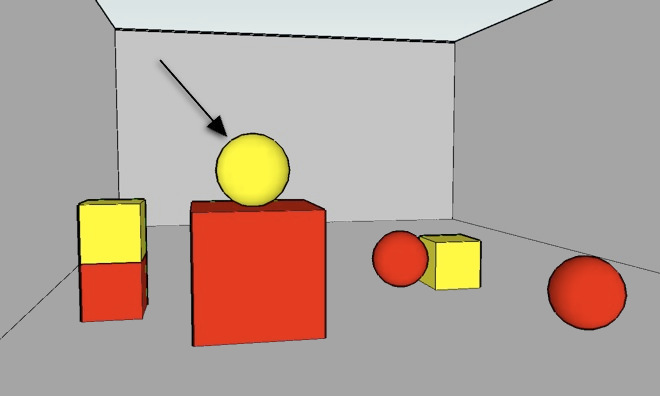
\includegraphics[width=0.6\textwidth]{images/7.jpg}
\caption{Ejemplo de contexto del corpus GRE3D7}
\label{GRE3D7-stimulus7}
\end{figure}

Seg\'un \cite{pechmann} el color de un objeto es una propiedad preferida en ER minimales y sobreespecificadas. Y, en particular, en expresiones sobre-especificadas, \cite{time-course} muestran evidencia emp\'irica de que color es preferida antes que la propiedad de tama\~no.
Filtrando las ER que no son relacionales de 3 corpus seleccionados, \cite{gre3d3}, \cite{gre3d7} y Stars2 y habiendo una propiedad o relaci\'on discriminativa del landmark (siempre la hay en stars2), esta propiedad o relaci\'on es preferida para sobreespecificar la descripci\'on del landmark.
Usa el algoritmo incremental con relaciones \cite{incremental}, el cual da siempre una ER minimal, incluye relaciones como \'ultimo recurso cuando no pueden distinguir al target con las propiedades at\'omicas. Otro algoritmo que luego de hacer lo que hace el anterior, selecciona 1 propiedad m\'as para el landmark y \'esta, es la propiedad m\'as frecuente en la parte de entrenamiento de un corpus del dominio. Propone un algoritmo igual al primero al que luego le agrega una propiedad m\'as al landmark, la de mayor poder discriminativo. En caso de empate entre varias propiedades, selecciona la m\'as frecuente del corpus de entrenamiento y en caso de no haber propiedades discriminatorias, no selecciona ninguna, quedando como el primer algoritmo. Compara \cite{dice}, y Accuracy para los 3 algoritmos, para 2 de 3 corpus consigue que el tercer algoritmo mejore ambos, pero no para el GRE3D7. 
Explica que por la naturaleza del corpus GRE3D7, ya que solo el 50\% de los landmarks m\'as cercanos tiene una propiedad con alto nivel discriminativo, en vez en el corpus Stars2 todas tienen una propiedad con alto nivel discriminativo. Concluye que la propiedad o relaci\'on m\'as discriminativa ser\'a la propiedad preferida para el landmark cuando se ha decidido hacer sobreespecificaci\'on.

Dicen que como trabajo futuro se podr\'ia usar grados de discernibilidad, y esto es lo que usamos en esta tesis, luego en la Secci\'on \ref{sec:learning} usaremos la discernibilidad calculada como 1 sobre la cantidad de objetos que tienen la propiedad, en el contexto y la usaremos para calcular las probabilidades de uso de las palabras que le daremos al algoritmo.

%En nuestro trabajo para calcular las prob de uso de las palabras en el GRE3D7 , una de las propiedades fue la discriminacion, nosotros no encontramos tal correlación,  quizás por el mismo motivo q el dice (naturaleza del corpus)
%
%Me pregunto porque lo acotó a solo 1 propiedad y solo a la descripción del landmark
%Me gustaría probar q las prob de uso en el Start2, tienen fuerte correlación con la discriminacion.
%Me hubiera gustado q otro baseline en su trabajo fuera nuestro algoritmo...(me parece q tenia miedo)
%Nosotros tenemos una probabilidad de uso que nos sirve para agregar sobreespecificacion a la descripción del target y de los landmarks , no tenemos restricción de cantidad, podemos agregar varias.
%Los n\'umeros no son directamente comparables, ya q el filtro solo las relacionales y uso el total del corpus y nosotros usamos la mitad del corpus (solo verde, azul)



\subsection{Corpora de GER existente}
\label{sec:corpus2}
\label{sec:corpusTUNA}

%was the first prominent REG corpus to be made publicly available for research purposes. The corpus was developed in a series of general-purpose controlled experiments, containing 2280 descriptions produced by 60 speakers in two domains (1200 descriptions of furniture items and 1080 descriptions of people's photographs). TUNA does not contain relational descriptions, and it is possibly the only resource of this kind to include situations of reference to sets. The TUNA corpus has been extensively used in a series of shared tasks

{\bf TUNA} \cite{tuna-corpus} fue el primer corpus prominente para GER disponible p\'ublicamente con fines de investigaci\'on. El corpus fue desarrollado en una serie de experimentos controlados de prop\'osito general, contiene 2.280 descripciones producidas por 60 personas en dos dominios (1.200 expresiones referenciales de im\'agenes de muebles y 1080 expresiones referenciales de fotograf\'ias de personas situadas en una grilla). Se muestran ejemplos de im\'agenes en Figura \ref{imagenes-tuna}. El corpus TUNA no contiene descripciones relacionales, y es posiblemente el \'unico recurso de este tipo que incluye situaciones de referencia a conjuntos. Este corpus se ha utilizado ampliamente en una serie de desaf\'ios \cite{reg2009}. \\


%\begin{figure}[H]
%\begin{subfigure}{.5\textwidth}
  %\centering
%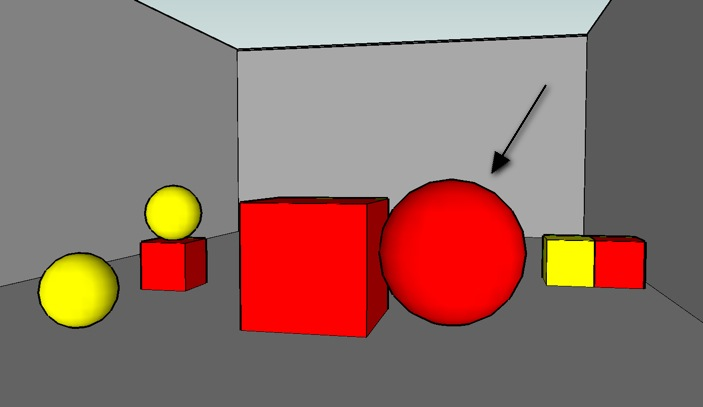
\includegraphics[width=\textwidth]{images/22sinletras.jpg}
  %\caption{}\label{GRE3D7-stimulus1}
%\end{subfigure}%
%\begin{subfigure}{.5\textwidth}




\begin{figure}[!ht]
\begin{subfigure}{.5\textwidth}
%\begin{minipage}[H]{0.5\linewidth}
\centering
\vspace*{.1cm}
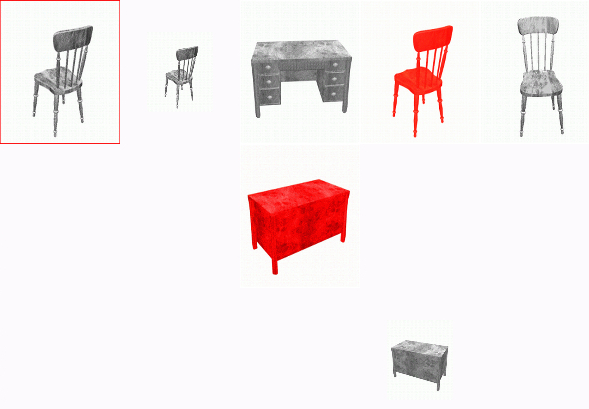
\includegraphics[width=\textwidth]{images/largeGreyChair.jpg}\\[0pt]
\caption{}
\label{fig-TUNA-furniture}
%\vspace*{.1cm}
\end{subfigure}
\hspace*{0cm}
\begin{subfigure}{.5\textwidth}
%\begin{minipage}[H]{0.5\linewidth}
\centering
\vspace*{-.8cm}
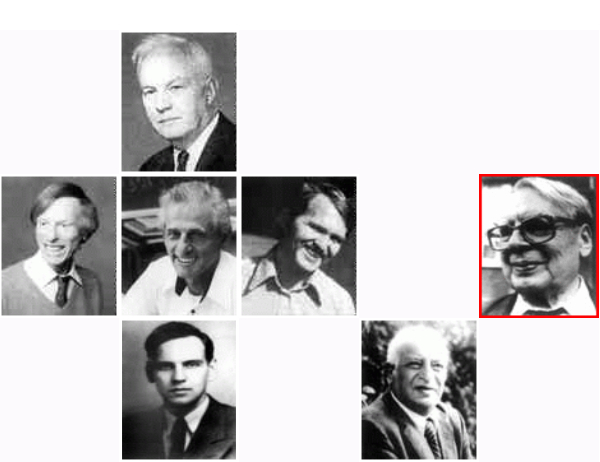
\includegraphics[width=\textwidth]{images/tuna-people.jpg}\\[0pt]
\caption{}
\label{fig-TUNA-people}
\end{subfigure}
\caption{Im\'agenes del TUNA corpus}\label{imagenes-tuna}
\end{figure}


\label{sec:corpusGRE}
%were developed in a series of web-based experiments primarily focussed on the study of relational descriptions. GRE3D3 contains 630 descriptions produced by 63 speakers, and GRE3D7 contains 4480 descriptions produced by 287 speakers, making it the largest of its kind to date. The GRE3D domain consists of simple visual scenes containing only two kinds of objects (boxes and spheres) with limited variation in colour and size. In each scene, there is only one possible spatial relation between target and the nearest landmark. Both corpora contain atomic and relational descriptions.
{\bf GRE3D3} y su extensi\'on {\bf GRE3D7} \cite{gre3d3,gre3d7} se desarrollaron en una serie de experimentos basados en la web, se centraron principalmente en el estudio de las descripciones relacionales. GRE3D3 contiene 630 descripciones producidas por 63 personas y GRE3D7 contiene 4.480 descripciones producidas por 287 personas, y es el corpus m\'as grande de este tipo hasta la fecha. El dominio del GRE3D3 consta de escenas visuales simples que contienen s\'olo dos tipos de objetos (cubos y esferas) con variaci\'on limitada en color y tama\~no. En cada escena, s\'olo hay una posible relaci\'on espacial entre el target y el landmark m\'as cercano. Ambos corpus contienen descripciones proposicionales y relacionales. Ejemplo de im\'agenes del GRE3D3 y GRE3D7 se muestran en la Figura \ref{imagenes-GRE3D3-GRE3D7}.
%\begin{minipage}[b]{0.45\linewidth}

\begin{figure}[!ht]
\begin{subfigure}{.35\textwidth}
\centering
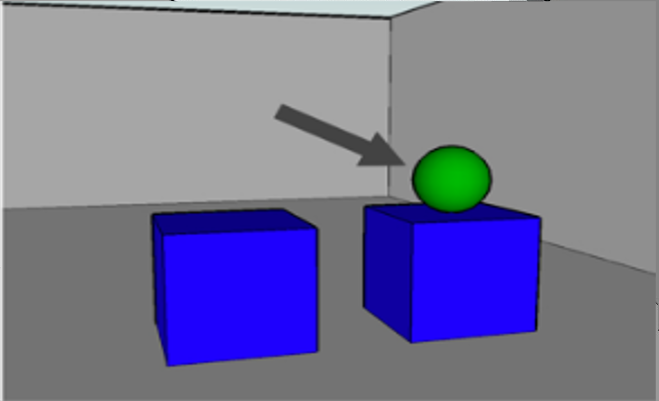
\includegraphics[width=\textwidth]{images/GRE3D3.png}\\[0pt]
\caption{}
\label{fig-GRE3D3}
%\vspace*{-0.7cm}
\end{subfigure}
\hspace*{0cm}
\begin{subfigure}{.65\textwidth}

\centering
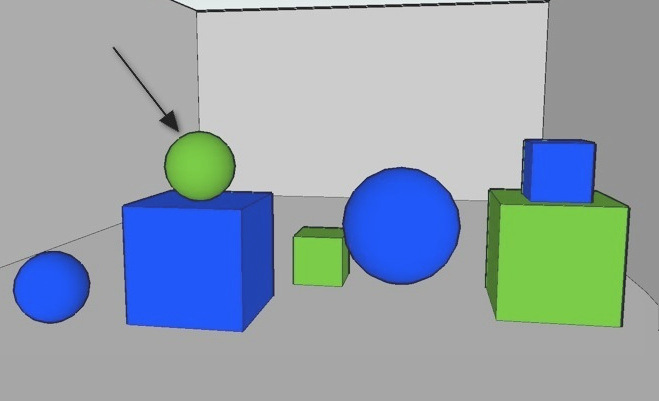
\includegraphics[width=\textwidth]{images/3.jpg}\\[0pt]
\caption{}
\label{fig-GRE3D7}
\end{subfigure}
\caption{Im\'agenes del GRE3D3/7}\label{imagenes-GRE3D3-GRE3D7}
\end{figure}

\vspace*{1cm}

\label{sec:corpusSTARS}
%and its extension Stars2 were collected for the study of referential overspecification (particularly in the case of relational descriptions). Stars was developed in a pilot web-based experiment, containing 704 descriptions produced by 64 speakers.  The more comprehensive Stars2 data set was produced in dialogue situations involving subject pairs, and it contains 884 descriptions produced by 56 speakers. Both domains make use of simple visual scenes containing up to four object types (e.g., stars, boxes, cones and spheres) with limited variation in colour and size. Differently from other REG corpora, however, Stars/2 includes a considerable number of complex situations of reference involving up to three objects, as in `the box near the sphere, next to the cone'.http://ppgsi.each.usp.br/arquivos/RelTec/PPgSI-002_2014.pdf y http://ppgsi.each.usp.br/arquivos/RelTec/PPgSI-001_2015.pdf
{\bf Stars} \cite{stars-mutual-disamb} y su extensi\'on {\bf Stars2} se recolectaron para el estudio de la sobre-especificaci\'on (particularmente en el caso de las descripciones relacionales). Stars se desarroll\'o en un experimento piloto basado en la web, contiene 704 descripciones producidas por 64 personas. El conjunto de datos Stars2 se obtuvo de situaciones de di\'alogo que implicaban a dos personas, contiene 884 descripciones producidas por 56 participantes. Ambos dominios hacen uso de escenas visuales simples que contienen tres tipos de objetos (por ejemplo para Stars, estrellas, cuadrados y c\'irculos y para Stars2 cubos, conos y esferas) con variaci\'on limitada en color y tama\~no. A diferencia de otros corpus para GER, Stars/2 incluyen un n\'umero considerable de situaciones complejas de referencia en que participan hasta tres objetos, como en {\it el cubo cerca de la esfera, al lado del cono}. Ejemplos de im\'agenes se muestran en la Figura \ref{imagenes-stars-stars2}.

\begin{figure}[!ht]
\begin{subfigure}{.5\textwidth}

\centering
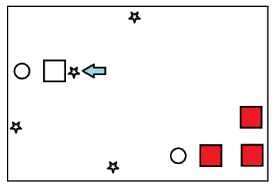
\includegraphics[width=\textwidth]{images/STARS.png}\\[0pt]
\caption{}
\label{fig-STARS}
%\vspace*{1cm}
\end{subfigure}
\hspace*{0cm}
\begin{subfigure}{.5\textwidth}

\centering
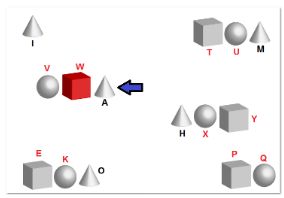
\includegraphics[width=\textwidth]{images/STARS2.png}\\[0pt]
\caption{}
\label{fig-STARS2}
\end{subfigure}
\caption{Im\'agenes de Stars/2 corpus}\label{imagenes-stars-stars2}
\end{figure}


\label{sec:corpusZOOM}
%were developed in a series of web-based experiments primarily focussed on the study of relational descriptions. GRE3D3 contains 630 descriptions produced by 63 speakers, and GRE3D7 contains 4480 descriptions produced by 287 speakers, making it the largest of its kind to date. The GRE3D domain consists of simple visual scenes containing only two kinds of objects (boxes and spheres) with limited variation in colour and size. In each scene, there is only one possible spatial relation between target and the nearest landmark. Both corpora contain atomic and relational descriptions.
El {\bf ZOOM} corpus se desarrollar\'o en un trabajo conjunto con la Universidad de S\~ao Paulo, contiene ER para 20 mapas de las ciudades de Lisboa y Madrid, fue realizado en la web, y contiene ER de targets singulares y plurales, con y sin zoom, en 2 idiomas: espa\~nol y portugu\'es. El corpus portugues contiene 100 ER por mapa, es decir 2000 ER en total, y el espa\~nol 80 por mapa, sumando un total de 1600 ER. El corpus fue recolectado a fin de poder realizar experimentos con situaciones mucho m\'as naturales que los corpus existentes hasta el momento. Ejemplos de mapas se muestran en la Figura \ref{imagenes-zoom-corpus}.


%\begin{figure}[!ht]
%\begin{minipage}[b]{0.46\linewidth}
%\centering
%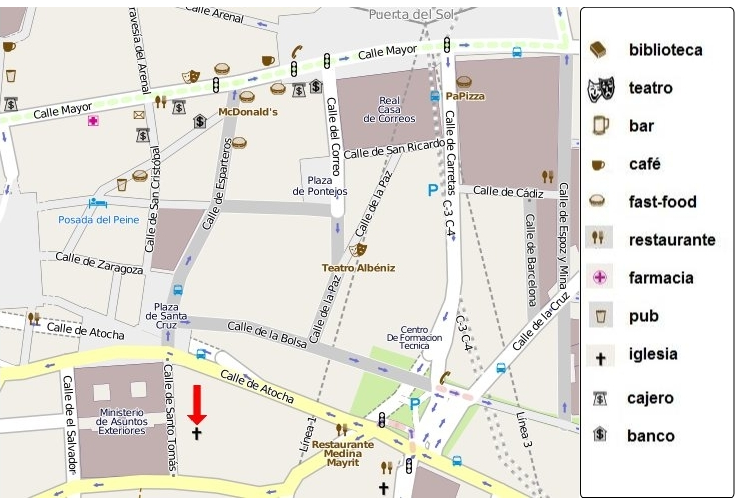
\includegraphics[width=\textwidth]{images/corpus/mapa6.png}\\[0pt]
%\caption{Target singular con zoom X}
%\label{singularx}
%\end{minipage}
%%\vspace*{.1cm}
%\begin{minipage}[b]{0.54\linewidth}
%\centering
%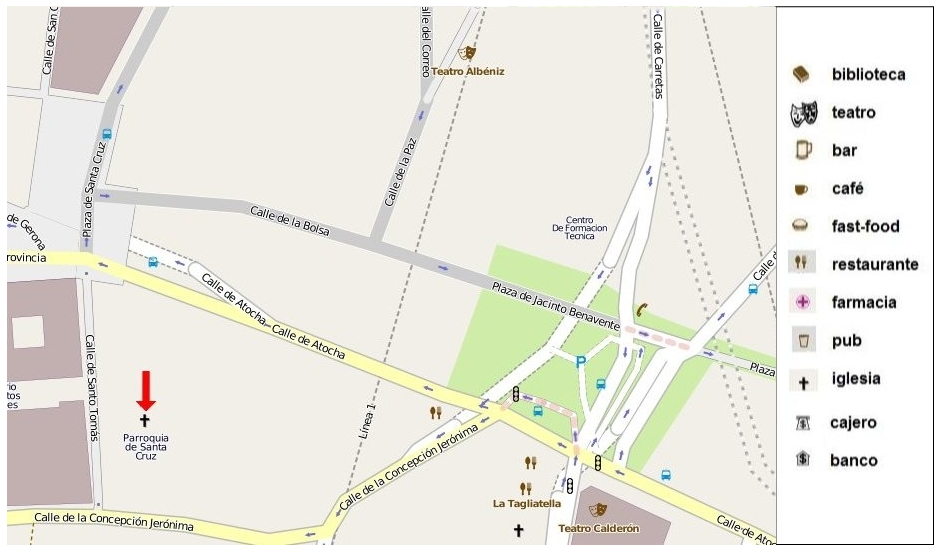
\includegraphics[width=\textwidth]{images/corpus/mapa16.png}\\[0pt]
%\caption{Target singular con zoom 2X}
%\label{singular2x}
%\end{minipage}
%\end{figure}

\begin{figure}[!ht]
\begin{subfigure}{.47\textwidth}
\centering
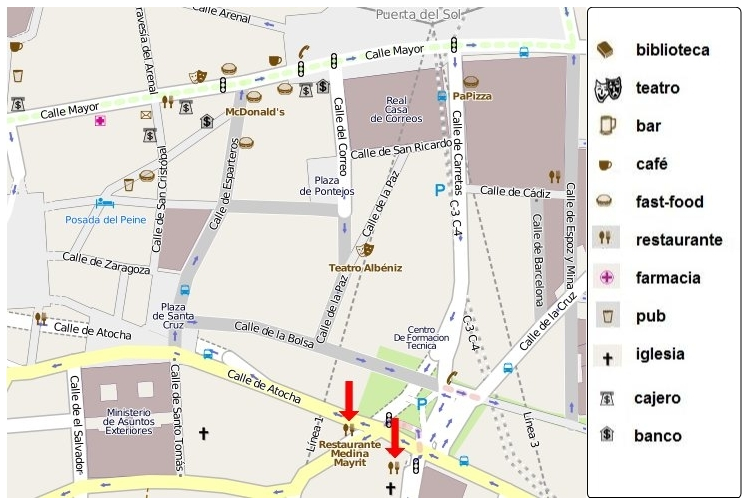
\includegraphics[width=\textwidth]{images/corpus/mapa10.png}\\[0pt]
\caption{}
\label{pluralx}
\end{subfigure}
%\vspace*{.1cm}
\begin{subfigure}{.53\textwidth}
\centering
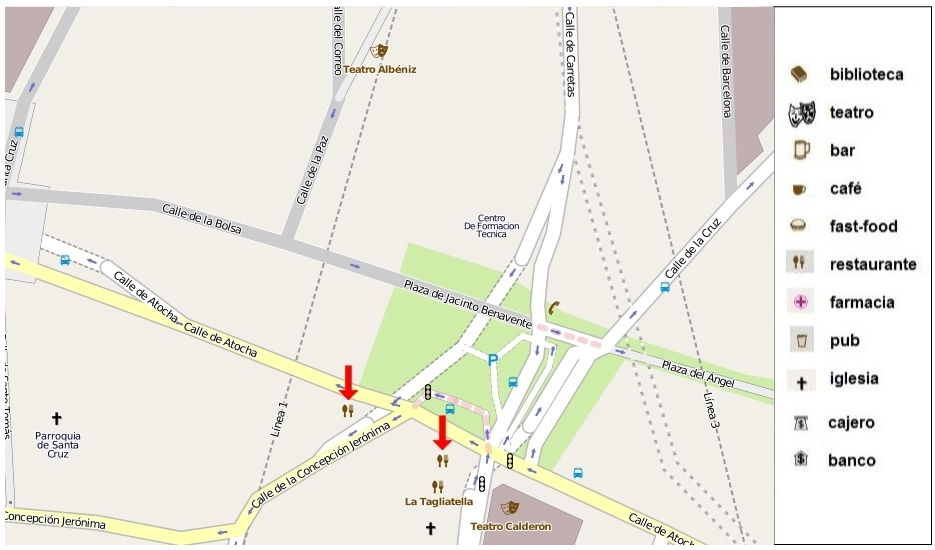
\includegraphics[width=\textwidth]{images/corpus/mapa20.png}\\[0pt]
\caption{}
\label{plural2x}
\end{subfigure}
\caption{Im\'agenes del ZOOM corpus, target plural sin zoom (izquierda) y con zoom (derecha)}\label{imagenes-zoom-corpus}
\end{figure}

En la Tabla \ref{tab-comparison} se comparan los diferentes corpus presentados anteriormente\footnote{En el caso del TUNA corpus se us\'o para la comparaci\'on s\'olo la parte singular.}, el n\'umero de propiedades diferentes que tiene en cuenta cada corpus se muestra en columna 'Propiedades'. El n\'umero de posibles landmarks que la descripci\'on puede incluir se muestra en la columna 'Landmarks', el largo promedio de la ER, en el sentido de la cantidad de atributos y relaciones, se ve en la columna 'Largo promedio' y la proporci\'on de propiedades usadas, lo cual es la proporci\'on de propiedades que aparecen en la descripci\'on sobre el n\'umero total de posibles propiedades y landmarks en la columna 'Uso'. Mayores largos de descripci\'on y menor promedio de uso se ven en situaciones complejas de referencia.
  %the average description size (in number of annotated properties), and the proportion of property usage, which is taken to be  the proportion of properties that appear in the description over the total number of possible attributes and landmarks. From a REG perspective, larger description sizes and lower usage rates are likely to represent more complex situations of reference.

\begin{table}[ht]
\begin{center}
\footnotesize{
\caption{Compaci\'on de corpora GER existente}
\label{tab-comparison}
\begin{tabular} {  l c c c c}
\hline
Corpus											&Propiedades			  & Landmarks			& Largo promedio	& Uso \\
\hline
TUNA-Muebles							  & 4								& 0							&	3.1				& 0.8   \\
TUNA-Personas								& 10							& 0							& 3.1				& 0.3   \\
GRE3D3											&	9								& 1							& 3.4				& 0.3   \\
GRE3D7											&	6								& 1							& 3.0				& 0.4   \\
Stars												&	8								& 2							& 4.4				& 0.4   \\
Stars2											& 9								& 2							& 3.3				& 0.3   \\
Zoom-Portugu\'es						& 19							& 4							& 6.7				& 0.3   \\
Zoom-Espa\~nol							& 19							& 4							& 7.2				& 0.3   \\
\hline
\end{tabular}
}
\end{center}
\end{table}

\cite{viethen-phd} dice que hay tres \'areas principales en las que los corpus se puede utilizar para
promover el objetivo de la semejanza humana en la investigaci\'on sobre generaci\'on de expresiones referenciales:
evaluaci\'on, la recolecci\'on de corpus y an\'alisis y modelizaci\'on estad\'istica de
datos de corpus.
Comenz\'o con el an\'alisis del estado del arte de la investigaci\'on en
la generaci\'on de descripciones distintivas, trabaj\'o con relaciones espaciales y en el trabajo us\'o datos de corpus. Examin\'o una serie de opciones metodol\'ogicas que tienen que hacerse cuando se trabaja con los corpus de GER. Aqu\'i, explor\'o diferentes opciones para los desaf\'ios de recopilaci\'on de corpus, que se centran en torno al equilibrio que se necesita
entre el control de los par\'ametros experimentales tanto como sea necesario
y mantener la configuraci\'on de lo m\'as natural posible. Discuti\'o una serie de conceptos
que son de importancia para el an\'alisis de corpora de GER, tales como la naturalidad de diferentes
propiedades de los objetos, y las nociones de minimalidad y cuestiones de sobre-especificaci\'on de expresiones referenciales. Por \'ultimo, analiz\'o diferentes maneras en que la salida de un sistema se puede
comparar con los datos de corpora, bajo la premisa de que el objetivo de la comparaci\'on es
para evaluar si el sistema podr\'ia tener un modelo adecuado del comportamiento humano para la generaci\'on de expresiones referenciales.
Realiz\'o una investigaci\'on en las tres \'areas donde se puede emplear corpora en GER: Evaluaci\'on de semejanza humana, recopilaci\'on y an\'alisis de corpus, y modelado de datos de corpus. Realiz\'o un experimento de evaluaci\'on con tres de los algoritmos cl\'asicos, (1989) Algoritmo Greedy de Dale (Greedy), Dale y Haddock (1991b), Algoritmo Relacional (ra) Y Dale y Reiter (1995) Algoritmo Incremental (IA), Se pusieron a prueba en cuanto a su capacidad de
replicar las expresiones referenciales se encuentran en un grupo relativamente peque\~no de corpus de expresiones referenciales
en un dominio visual de im\'agenes puestas en una grilla.
%de rejilla de cajones de armarios ling. 
En el an\'alisis de este experimento tuvo dos resultados principales: (1) que identic\'o en particular tres 
fen\'omenos que todav\'ia plantean importantes retos para los algoritmos GER con el objetivo de replicar
el comportamiento humano, y (2) que proporciona una plataforma para la discusi\'on de una serie de
dificultades que se presentan para la evaluaci\'on basada en corpus de GER. Esto result\'o en una serie
de criterios para el dise\~no de los dos corpus que el trabajo en el resto de la tesis.
Los tres fen\'omenos en las expresiones referenciales producidas por humanos que los
algoritmos probados no fueron capaces de replicar satisfactoriamente sobre-especificaci\'on,
relaciones espaciales, y comportamiento de voluntarios espec\'ificos. Ambos
Greddy y la IA fueron capaces de generar algo de la redundancia que se encontr\'o en el corpus.
 Ni Greedy ni el IA estaban dise\~nados para ser capaz de generar expresiones referenciales que contengan relaciones entre entidades, pero el ra fue dise\~nado para incluirlas. Sorprendentemente, el
ra no s\'olo fallo en generar cualquiera de las descripciones contenidas en el corpus de evaluaci\'on; sino tambi\'en que las descripciones que se gener\'o parec\'ian m\'as como enigmas cuyo objetivo era confundir a un oyente, m\'as que ayudar en
los intentos de se\~nalar el objetivo referente. 

Una valoraci\'on te\'orica de otras aproximaciones dise\~nados para manejar las relaciones estableci\'o que ninguno de ellos incluir\'ia una relaci\'on, si no es absolutamente necesaria para distinguir el target.
La tercera observaci\'on que el experimento dejo a la vista fue que la gente no siempre hace lo mismo en la misma situaci\'on. De hecho, incluso la misma persona podr\'ia describir el mismo target de diferente manera en distintas
circunstancias. 





\section{Generaci\'on \emph{autom\'atica} de expresiones referenciales}
\label{sec:tipos_algoritmos}

Un algoritmo para la generaci\'on autom\'atica de expresiones referenciales es un programa que dado un input d\'a una ER para un target.

Los algoritmos pueden ser de distintos tipos, seg\'un los tipos de ER que sean capaces de generar. Por ejemplo, un algoritmo puede ser: determin\'{i}stico o no-determin\'{i}stico, relacional o proposicional, incluir negaciones o no, generar plurales, singulares o ambos,
 %usar disyunciones y conjunciones, o s\'olo conjunciones, 
generar ER sobreespecificadas o minimales. A continuaci\'on se describen cada uno de esos tipos.

Un algoritmo es {\bf determin\'{i}stico} si dado un input (un contexto y un target), d\'a siempre la misma ER de salida. En cambio, un algoritmo es {\bf no-determin\'{i}stico} si es posible que d\'e distintas salidas para el mismo input, en distintas ejecuciones. En general las personas generan expresiones referenciales de forma no determin\'istica, en este sentido los algoritmos no-determin\'isticos simulan el comportamiento de las personas. 

Por ejemplo, un algoritmo no determin\'istico podr\'ia generar para la Figura \ref{GRE3D7-stimulus}, una vez {\it La esfera roja} y otra vez {\it La esfera grande}. En la Tabla \ref{er-gre3d7-stimulus} se muestran las distintas ERs dadas por las personas para la Figura \ref{GRE3D7-stimulus} del corpus GRE3D7 \cite{gre3d7}. La tabla tambi\'en muestra cu\'antas personas generaron esa ER para el target de la figura. Por ejemplo {\it large red ball} ocurri\'o 71 veces en el corpus, es decir m\'as de la mitad de las personas decidieron incluir el tipo, el tama\~no y el color en su ER, generando as\'i una ER sobreespecificada.

%Si el algoritmo es determin\'istico dar\'ia s\'olo una ER. ?`Esa ER que dar\'ia el algoritmo coincidir\'a con alguna de las que dieron las personas?. 
%Si el algoritmo es no-determin\'istico, ?`podremos conseguir todos los diferentes tipos de ER que dieron las personas?. %Intentaremos responder estas preguntas m\'as adelante en la tesis.\\
Si el largo de la ER es finito, dado un contexto finito, existen finitas ER a generar, as\'i un algoritmo no-determin\'istico nos permitir\'ia explorar todas las ER posibles para un input dado.

\begin{table}[h!]
\begin{center}
\begin{tabular}{|c|l|c|}
\hline
%total scenes in evaluation set &                           80   &             68
 Orden&ER& Cantidad \\
\hline
1&large red ball & 71 \\
2&red ball & 56 \\ 
3&large red ball next-to large red cube & 5 \\ 
4&large ball & 2 \\ 
5&large red ball next-to red cube & 2 \\ 
6&large red ball right-of large red cube & 1 \\ 
7&large red ball next-to large red ball & 1 \\ 
8&large red ball next-to cube & 1 \\ 
9&red ball next-to large red cube & 1 \\ \hline
Total & &140 \\ \hline
\end{tabular}
%\vspace*{.1cm}
\caption{ER dadas por las personas para la Figura \ref{GRE3D7-stimulus} del corpus GRE3D7.} 
\label{er-gre3d7-stimulus}
\vspace*{-.5cm}
\end{center}
\end{table}

Un algoritmo es {\bf proposicional}, cuando las ERs que genera contienen s\'olo atributos del target, es decir no contiene relaciones con otros objetos ni propiedades de otros objetos. Por ejemplo, s\'olo podr\'ia generar las ER 1, 2 y 4 de la Tabla \ref{er-gre3d7-stimulus}. Es decir, genera solamente ERs proposicionales.

Un algoritmo es {\bf relacional} si adem\'as de generar ERs proposicionales genera ERs relacionales, en cuyo caso adem\'as de generar las relaciones correspondientes deber\'a generar expresiones para \'el o los objetos relacionados. Un algoritmo relacional podr\'ia generar todas las ERs de la Tabla \ref{er-gre3d7-stimulus}. Es interesante notar que no todas las descripciones de los objetos involucrados en una ER relacional, son ER que identifican un\'ivocamente al objeto. Por ejemplo, consideremos la ER 8, {\it La gran esfera roja a la derecha del cubo}. En este caso, {\it el cubo} es una expresi\'on que se tuvo que dar como consecuencia de incluir la relaci\'on {\it a la derecha de}. La expresi\'on {\it el cubo} no es una ER. 

En algunos contextos, por ejemplo cuando el target es el \'unico que no tiene una propiedad o relaci\'on, ser\'ia \'util un algoritmo que incluya {\bf negaciones}. Por ejemplo, para la Figura \ref{GRE3D7-stimulus}, la ER {\it La esfera que est\'a sola} podr\'ia ser 
una forma efectiva de referirse a $e_1$ dado que es la \'unica esfera que no est\'a tocado un cubo.

Un algoritmo puede generar ER para un conjunto de objetos en el contexto considerado. Por ejemplo, para la Figura \ref{GRE3D7-stimulus} la ER {\it Los cubos} se refiere al conjunto de objetos \{$e_2$, $e_4$, $e_6$, $e_7$\}. Estos algoritmos generan ER {\bf plurales}. En caso de no poder generar ER para un target no singleton se dice que el algoritmo genera s\'olo {\bf singulares}.

Un algoritmo que genera ER {\bf minimales} (que se explicaron en la Secci\'on \ref{sec:minimales}), es un algoritmo que d\'a ERs que contienen la m\'inima cantidad de propiedades o relaciones que se necesitan para distinguir al target. Por ejemplo, en la Tabla \ref{er-gre3d7-stimulus} las ER 2 y 4 son minimales. Normalmente, si el algoritmo es determin\'istico entonces un orden preferencial de las propiedades tomado como input hace que el algoritmo pueda decidir cu\'al ER dar en caso de tener varias minimales.

Un algoritmo que haga {\bf sobreespecificaci\'on} tiene la caracter\'istica de poder dar m\'as propiedades o relaciones con otros objetos que las m\'inimas necesarias para identificar al target. Por ejemplo, para la Figura \ref{GRE3D7-stimulus} la ER {\it La esfera roja, grande que esta a la derecha del cubo rojo grande} es una ER sobreespecificada porque (como ya mencionamos en la Secci\'on \ref{er-sobreespecificadas}) podr\'iamos sacarle algunas propiedades o la relaci\'on y seguir\'ia siendo una ER. Sacando {\it roja} de las propiedades del target, la expresi\'on {\it La esfera grande que esta a la derecha del cubo rojo grande} sigue siendo una ER, tambi\'en podr\'iamos sacar la relaci\'on con {\it el cubo rojo grande}, quedando {\it La esfera roja, grande} y sigue siendo una ER. Viendo la Tabla \ref{er-gre3d7-stimulus} podemos notar que la ER de mayor frecuencia, es {\it large red ball} y es una ER sobreespecificada, ya que {\it red ball} o {\it large ball}, son ERs minimales para el target de la Figura \ref{GRE3D7-stimulus}. En la tabla hay 58 ER minimales y 82 sobreespecificadas. Es decir, el 58\% son sobreespecificadas y el 41\% minimales.

Hay una forma trivial de que un algoritmo sobreespecifique: agregar todas las propiedades y relaciones del target con otros objetos. Por ejemplo, para la Figura \ref{GRE3D7-stimulus} la ER ser\'ia {\it Large red ball left-of (large red cube right-of large red ball)}. Pero, como vemos en la Tabla \ref{er-gre3d7-stimulus}, esto no es lo que hace la gente. En esta tesis, uno de los temas que investigamos es c\'omo hacer para el que un algoritmo sobreespecifique imitando el comportamiento humano lo m\'as posible. 

Los algoritmos no generan expresiones parciales ni subespecificadas, ya que no sirven para identificar al target. La identificaci\'on del target es el objetivo de la GER.


%\section{Algoritmos importantes en el \'area}

%interesante...
%https://www.abdn.ac.uk/ncs/departments/computing-science/tunabibl-495.php


Ahora vamos a hablar de una selecci\'on de algoritmos de generaci\'on autom\'atica de expresiones referenciales del \'area. En la Tabla \ref{clasificacion_algoritmos} se muestra una clasificaci\'on seg\'un los tipos de algoritmos que vimos en la secci\'on anterior, considerando si es determin\'istico o no-determin\'istico, proposicional o relacional, si genera negaciones, plurales, si genera sobreespecificaci\'on. Notar que si no generan sobreespecificaci\'on, generan ERs minimales.

\subsection{Primeros algoritmos}

\label{sec:algoritmos_area}

\begin{table}[h!]
\begin{center}
\begin{tabular}{|l|c|c|c|c|c|c|c|}
\hline
%total scenes in evaluation set &                           80   &             68
 Algoritmos& Deter- & No-Deter & Propo- & Re- & Nega- & Plu- & Sobre- \\
 & min\'istico & min\'istico & sicional & lacional & ciones & rales & especificado \\
 %Algoritmos& Det. & No-Det. & Prop. & Rel. & Neg. & Plur. & Sob. \\
\hline
Full Brevity &Si & No&Si&No&No&No& No \\
Greedy&Si & No&Si&No&No&No& Si \\
Incremental&Si & No&Si&No&No&No& No \\
GRAPH&Si & No&Si&Si&No&Si& Si \\ \hline
%Bisimulaci\'on&Si & No&Si&Si&Si&Si& No \\ \hline
%Nuestra Propuesta&No & Si&Si&Si&No&Si& Si \\

\end{tabular}
%\vspace*{.1cm}
\caption{Clasificaci\'on de algoritmos seg\'un el tipo de ER que generan.} 
\label{clasificacion_algoritmos}
\vspace*{-.5cm}
\end{center}
\end{table}


 
%survey
%http://citeseerx.ist.psu.edu/viewdoc/download?doi=10.1.1.227.8284&rep=rep1&type=pdf


\paragraph{Full brevity:} El algoritmo {\bf Full Brevity} \cite{Dale:1989:CUR:981623.981632} genera la descripci\'on m\'as corta que identifica al target. Para hacerlo, 
busca si hay una propiedad del target que no sea propiedad de ning\'un distractor. Si no hay chequea todas las posibles combinaciones de 2 propiedades, si no la hay, busca de a 3 y as\'i sucesivamente. Por ejemplo para la Figura \ref{GRE3D7-stimulus} se fijar\'ia en las propiedades del target {red, ball, large}, como ninguna de ellas aisladamente identifica s\'olo al target, probar\'ia con 2 propiedades {\it red ball} si identifica al target, devuelve {\it red ball} y finaliza.

\paragraph{Heur\'istica Greedy:} Una aproximaci\'on a Full Brevity es el algoritmo de {\bf Heur\'istica Greedy}, el cual iterativamente selecciona la propiedad que elimina m\'as distractores y argumentan que la propiedad seleccionada tiene el m\'as alto poder discriminativo en esa etapa. Como resultado no siempre genera expresiones referenciales m\'inimas.

El problema es que encontrar la descripci\'on m\'as corta es computacionalmente caro, se observ\'o que las personas dan expresiones que no son minimales, esto fue confirmado por estudios psycoling\"uisticos \cite{Olson1970LangAndThought};  \cite{Sonnenschein1984}; \cite{Pechmann1989}.

El algoritmo de heur\'istica Greedy es m\'as eficiente que el Full Brevity, pero pronto fue superado por el algoritmo {\it Incremental} y sus sucesores \cite{C92-1038}; \cite{Dale95computationalinterpretations}. El algoritmo Incremental fue y sigue siendo uno de los algoritmos m\'as importantes del \'area, lo explicamos a continuaci\'on. Por ejemplo para la Figura \ref{GRE3D7-stimulus} se fijar\'a que {\it ball} elimina 2 distractores {$e_{1}$, $e_{3}$}, {\it red} elimina 3 distractores {$e_{2}$, $e_{4}$, $e_{7}$} y {\it large} elimina 1 distractores {$e_{4}$}, entonces elegir\'a {\it red}, pero como no alcanza para ser ER, seguir\'a con {\it ball} que es la que elimina m\'as distractores luego de {\it red}, finalizar\'a porque {\it red ball} identifica al target. Supongamos que hubiera otro objeto con propiedad {\it large}, entonces {\it large} eliminar\'ia tambi\'en 2 distractores, entonces el algoritmo devolver\'ia {\it large red ball}, y esa ER no es minimal, es sobreespecificada.

\paragraph{Incremental:}

\begin{figure}[ht]
%\centering
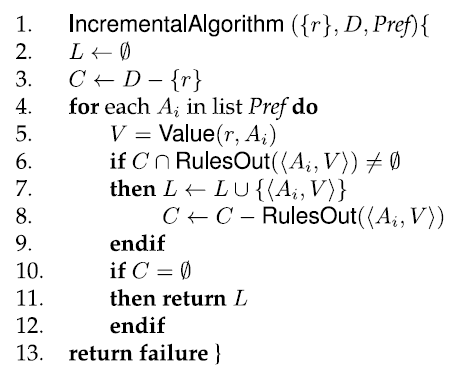
\includegraphics[width=.5\textwidth]{images/algoritmoIncremental.png}
%\caption{Algoritmo Incremental}
\label{algoritmoIncremental}
\caption{Figura 2 de \protect\cite{survey}}
\end{figure}

%\begin{figure}[ht]
%%\centering
%\includegraphics[width=0.6\textwidth]{images/algIncremental.png}
%%\caption{Algoritmo Incremental}
%\label{algoritmoIncremental}
%\caption{Figura 2 de \protect\cite{survey}}
%\end{figure}

El input del {\bf Algoritmo Incremental}, es el target \emph{r}, que queremos identificar, $e_{5}$, \emph{D} es el dominio, y \emph{Pref} una lista de propiedades ordenada seg\'un la preferencia. Vamos a ejemplificar la corrida del algoritmo con el ejemplo de la Figura \ref{GRE3D7-stimulus}, y supongamos que la lista ordenada de propiedades es \'esta [ tipo, color, tama\~no ]. \emph{D} inicialmente es el conjunto de todos los objetos del contexto: \{$e_{1}$,$e_{2}$,$e_{3}$,$e_{4}$,$e_{5}$,$e_{6}$,$e_{7}$\}.
En {\it Paso 2} se asigna a \emph{L} la descripci\'on vac\'{i}a, al finalizar la ejecuci\'on, \emph{L} tendr\'a el conjunto de propiedades con los cuales identificaremos a \emph{r}. Se inicializa \emph{C} con el conjunto de distractores de \emph{r} en nuestro ejemplo \{$e_{1}$,$e_{2}$,$e_{3}$,$e_{4}$,$e_{6}$,$e_{7}$\}, en el {\it Paso 3}. 
La idea del algoritmo es ir eliminando distractores, por eso, en el {\it Paso 4} recorre las propiedades $A_{i}$ de \emph{r}. En {\it Paso 5} le asigna a \emph{V} el valor que tiene la propiedad $A_{i}$ para el target \emph{r}, $RulesOut(A_{i},V)$ es el conjunto de objetos que tienen diferente valor para la propiedad $A_{i}$ que el que tiene el  target, la funci\'on se fija si el valor de esa propiedad elimina distractores. La primer propiedad de \emph{r} a considerar seg\'un el orden de preferencias \emph{Pref} es ``tipo'', el valor del target para tipo es {\it esfera}, entonces en {\it Paso 6}, pregunta si hay objetos en \emph{C} que tengan tipo con valor distinto de esfera, y hay, ellos son \{$e_{2}$,$e_{4}$,$e_{6}$,$e_{7}$\}, entonces le asigna a \emph{C} \{$e_{1}$,$e_{3}$\}, es decir s\'olo las que son esferas. En {\it Paso 10} pregunta si \emph{C} es vac\'io, es decir si ya se eliminaron todos los distractores, pero no lo es, por lo tanto continua con la siguiente propiedad, en este caso ``color'', el valor de color para el target es {\it rojo}, agrega {\it rojo} a \emph{L}, y actualiza \emph{C} con $\emptyset$ porque tanto $e_{1}$ como $e_{3}$ son amarillos, en {\it Paso 10} pregunta si \emph{C} es vac\'io, y si lo es, por lo tanto devuelve \{esfera, rojo\}. Lo cual se podr\'ia realizar como {\it La esfera roja}, y ser\'ia una ER para el target considerado.


Luego se propusieron extensiones del algoritmo Incremental, por ejemplo, una extensi\'on que permite la generaci\'on de referencia teniendo en cuenta la prominencia discurso del target \cite{Krahmer:2010:EMN:1880370}; \cite{krahmer-theune:2002a}; 
%y un segundo algoritmo que permite producir expresiones referenciales que contienen relaciones con otros objetos. El enfoque Theune y de Krahmer funciona asignando una puntuaci\'on de relevancia a todos los objetos de acuerdo con el enfoque / tema distinci\'on por \cite{hajicova-1993} y la teor\'ia de centrado \cite{Grosz:1995:CFM:211190.211198}. Alteran el criterio de \'exito del algoritmo y s\'olo permiten que se detenga cuando hay un distractor que es tanto o m\'as relevante que el target.
%No todas las propiedades tienen la misma relevancia. Las diferencias cualitativas que existen entre diferentes propiedades se discutieron por primera vez en la literatura GER por van Deemter (2000, 2006). Se\~nal\'o que la conveniencia de otras propiedades sobre las
%propiedades vagas como peque\~no y grande dependen del contexto en el que se utilizan, mientras que, por ejemplo, el color de un objeto es absoluta. 

\paragraph{Algoritmos relacionales}

%Various researchers have attempted to extend the IA by allowing relational descriptions
%(Horacek 1996; Krahmer and Theune 2002; Kelleher and Kruijff 2006), often based
%on the assumption that relational properties (like ``x is on y'') are less preferred than
%non-relational ones (like ``x is white''). If a relation is required to distinguish the target
%x, the basic algorithm is applied iteratively to y. It seems, however, that these attempts
%were only partly successful. One of the basic problems is that relational descriptions
%just like references to sets, but for different reasons do not seem to fit in well with an
%incremental generation strategy. In addition, it is far from clear that relational properties
%are always less preferred than non-relational ones (Viethen and Dale 2008). Viethen
%and Dale suggest that even in simple scenes, where objects can easily be distinguished
%without relations, participants still use relations frequently (in about one third of the
%trials).
Varios investigadores han intentado ampliar el algoritmo incremental permitiendo descripciones relacionales
(\cite{Horacek1997}; \cite{krahmer}; \cite{kelleher06:increm}), se basan a menudo
en el supuesto de que las propiedades relacionales (como ``x est\'a en y'') son menos preferidas que
los no relacionales (como ``x es blanca''). Si se requiere una relaci\'on para distinguir al target
x, en el cual se deba nombrar al objeto y, se aplica el algoritmo b\'asico iterativamente a y. Parece, sin embargo, que estos intentos
fueron s\'olo parcialmente exitosos. Uno de los problemas b\'asicos es que las descripciones relacionales
al igual que las referencias a conjuntos, pero por diferentes razones no parecen encajar bien con una
estrategia de generaci\'on progresiva. Adem\'as, no est\'a claro que las propiedades proposicionales sean siempre preferidas antes que las relacionales. En \cite{viet:gene11} se sugieren que, incluso en escenas simples, donde los objetos pueden f\'acilmente ser distinguidos
sin relaciones, las personas tambi\'en utilizan con frecuencia las relaciones (en aproximadamente un tercio de las ERs que dan).

Otra cosa interesante de mencionar es que en caso de generar ER relacionales hay que asegurarse que el algoritmo termina, es decir que no entra en loops tratando de identificar objetos. \cite{haddock} estudiaron como abordar el problema de regresi\'on infinita, en el cual el algoritmo trata de describir al landmark haciendo referencia al target, y al target haciendo referencia al landmark infinitamente, como en {\it el libro en la mesa la cual soporta un libro en la mesa... }



\subsection{Algoritmo de b\'usqueda en Grafo}
\label{graph}

%\begin{figure}[ht]
%\centering
%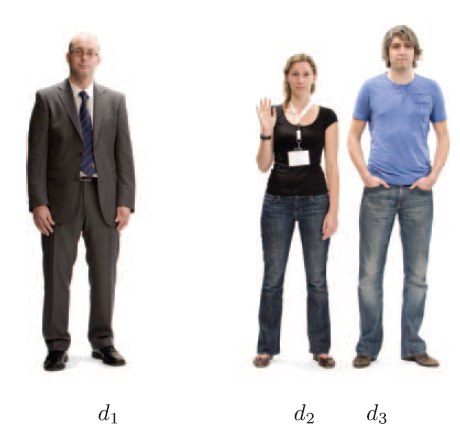
\includegraphics[width=0.4\textwidth]{images/contexto-survey.png}
%\caption{Ejemplo de contexto}
%\label{figura-survey}
%\end{figure}
%
%\begin{figure}[ht]
%\centering
%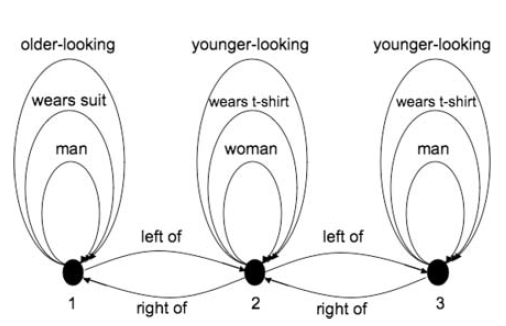
\includegraphics[width=0.4\textwidth]{images/grafo-survey.png}
%\caption{Ejemplo de grafo para el contexto de la Figura \ref{figura-survey}}
%\label{grafo-survey}
%\end{figure}





El {\bf algoritmo Graph} de \cite{Krahmer:2003} propone tratar la obtenci\'on de expresiones referenciales como un problema de grafos, el contexto que incluye al target y los distractores es representado como un grafo, por ejemplo para el contexto de la Figura \ref{figura-survey} el grafo correspondiente ser\'ia el de la Figura \ref{grafo-survey}. Cada objeto de la escena (personas en este caso) se modela como un v\'ertice en el grafo. Las propiedades at\'omicas como jounger-looking, older-looking, wears suit, wears t-shirt, woman, man, se representan como un bucle en el correspondiente nodo. Las relaciones binarias entre objetos, por ejemplo left-of o right-of se modelan como aristas entre los nodos correspondientes.

\begin{figure}[!ht]
\begin{subfigure}{.4\textwidth}\centering
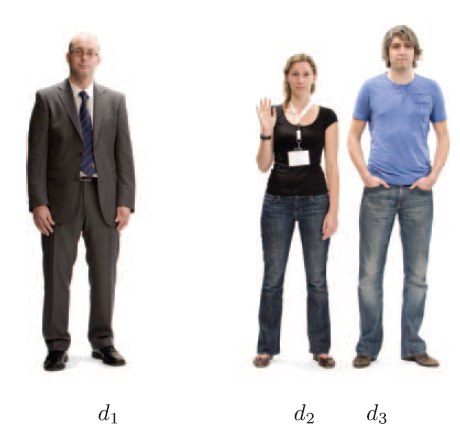
\includegraphics[width=\textwidth]{images/contexto-survey.png}\\[0pt]
\caption{}
\label{figura-survey}
\vspace*{.1cm}
\end{subfigure}
\hspace*{0cm}
\begin{subfigure}{.5\textwidth}\centering
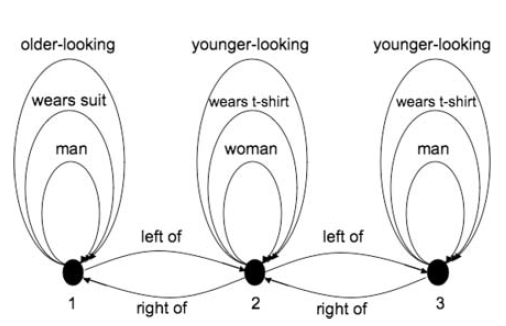
\includegraphics[width=\textwidth]{images/grafo-survey.png}\\[0pt]
\caption{Ejemplo de grafo para el contexto de la Figura \ref{figura-survey}}
\label{grafo-survey}
\end{subfigure}
\caption{Ejemplo de contexto y grafo extra\'ido de \protect\cite{survey}}

\end{figure}



Dado un objeto target, conseguir una ER que distinga al objeto de lo dem\'as es equivalente a encontrar un subgrafo del grafo original que unicamente caracterize al target. Intuitivamente este subgrafo se puede poner sobre el target y no sobre ningun otro objeto del dominio considerado.\\

\begin{figure}[ht]
\centering
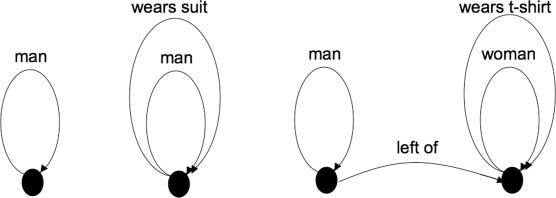
\includegraphics[width=0.6\textwidth]{images/ref-exp-graph.png}
\caption{Subgrafos de la Figura \ref{grafo-survey}}
\label{ref-exp-graph}
\end{figure}

%Para generar una descripci\'on distintiva, el algoritmo busca un subgrafo del grafo original que identifica al target un\'{i}vocamente al cual le llama grafo distintivo.% (distinguishing graph).\\
Comenzando con el subgrafo que contiene un solo v\'ertice, que representa al target, seg\'un una heur\'{i}stica basada en costos (costo de incluir propiedades, relaciones) empieza a agregar propiedades o relaciones, del target o nodos que ya hallan sido agregados. Cada vez que agrega algo, chequea si hay alg\'un otro nodo en el cual el grafo pueda distinguir, si lo hay quiere decir que es un distractor, cuando no hay el grafo distingue al target. Por ejemplo en la Figura \ref{ref-exp-graph} se ve el primer grafo {\it man}, el cual puede ser puesto sobre los nodos 1 y 3 de la Figura \ref{grafo-survey}, es decir no identifica s\'olo al target, el segundo grafo {\it man, wears suit} s\'olamente puede ser puesto sobre el nodo 1, por lo tanto es un grafo que distingue al target.  

El algoritmo sigue explorando grafos y siempre se queda con el de menor costo.

La funci\'on de costo esta definida sobre las aristas y v\'ertices del grafo dominio. El costo de un subgrafo se define como la suma sobre todas las aristas y v\'ertices que contiene el grafo.
El algoritmo de b\'usqueda garantiza encontrar el subgrafo de menor costo que representa al target.

La funci\'on de costo es usada para podar las ramas del \'arbol de b\'usqueda cuando estas se hacen m\'as costosas que el grafo de menor costo encontrado hasta el momento. Esta funci\'on hace que se prefieran propiedades sobre otras que tienen mayor costo.

%Por ejemplo, 
%Los algoritmos discutidos por Dale y Reiter (1995) pueden ser vistos como
%diferentes instancias de un algoritmo de b\'usqueda (Bohnet y Dale 2005; Gatt de 2007).
%Todos ellos, b\'asicamente, buscan a trav\'es de un mismo espacio de estados, compuestos por tres componentes: conjunto de cosas verdaderas para el target, un conjunto de distractores, y un conjunto de propiedades del target que a\'un no han sido consideradas. El estado inicial se puede formalizar como la tripla ($\emptyset$, C, P) 
%(no hay descripci\'on del target constru\'ida, no se han descartado distractores, y todas las propiedades P del target todav\'ia est\'an disponibles), y el estado final como
%(L, $\emptyset$, P'), se ha encontrado una descripci\'on que distingue al target,
%el conjunto de distractores est\'a vac\'io, y pueden o no quedar propiedades del target en P'. Todos los otros estados en el espacio de b\'usqueda son intermedios,
%a trav\'es de cuales un algoritmo podr\'ia moverse en funci\'on de su estrategia de b\'usqueda. 
%Por ejemplo 
%cuando buscamos de una descripci\'on distintiva de $e_{5}$ del Contexto\ref{GRE3D7-stimulus2}, un estado intermedio podr\'ia ser
%s = ({[forma, esfera],[color,rojo]},{$e_{5}$}, {[taman\~o, grande],[a-la-der-de, $e_4$]})
%
%Los algoritmos discutidos anteriormente difieren en el m\'etodo de creaci\'on de los estados, y en el orden en que estos estados son recorridos. Full Brevity, por ejemplo, utiliza un m\'etodo de expansi\'on, que crea un nuevo estado para cada atributo
%del target no contemplado antes (y que excluye al menos un distractor). 
%
%
%Comenzando desde el estado inicial y aplicando a nuestro ejemplo de contexto, este m\'etodo ser\'ia dar\'ia lugar a tres nuevos estados, la creaci\'on de descripciones, incluyendo la informaci\'on de forma, el color, y el taman\~o, respectivamente. Estos estados son chequeados mediante un m\'etodo de amplitud-primero. 
%El IA, por el contrario, utiliza un m\'etodo diferente para ampliar el grafo, cada vez que crea
%un nuevo estado, lo hace de acuerdo con un orden de preferencia predeterminado. As\'i, en
%el estado inicial, y suponiendo que (como antes) que escribe es el atributo m\'as preferido, el
%ampliar m\'etodo ser\'ia crear un solo nuevo estado: s = {[forma, esfera]}, siempre hay 1 solo nuevo estado elegido por el orden de preferencia.



%Considere dos descripciones de un dominio de los animales ... (van Deemter, 2002), van Deemter considera integridad l\'ogica del ia en t\'erminos de los operadores booleanos de negaci\'on y disyunci\'on. \'el la extendi\'o a
%ser capaz de generar expresiones referenciales que contienen propiedades, tales como Ejemplo (2.3) negado, y las descripciones de conjuntos de objetos, tales como Ejemplo (2.4), o incluso (2,5), que contiene una disyunci\'on l\'ogica de propiedades. Sus algoritmo procede
%en etapas, tratando m\'as y disyunciones m\'as largos de propiedades, si las propiedades at\'omicas
%y disyunciones m\'as cortos no son suficientes para distinguir el conjunto target .. que funciona en referencia a conjuntos fue tomada adem\'as por Gatt y van Deemter (2005, 2006), que han presentado los algoritmos m\'as maduros a la fecha. Utilizaron un procedimiento similar al de las otras cosas en que sus algoritmos se basan en el procesamiento incremental de un orden de preferencia de las propiedades. Sus algoritmos agregan una gran cantidad de maquinaria compleja para el procedimiento b\'asico para asegurar que las propiedades
%se eligen de manera que maximiza la coherencia dentro del conjunto de objetos descritos por las expresiones referenciales. Por ejemplo, su enfoque intentar\'a utilizar propiedades del mismo tipo para todos los referentes de un conjunto. As\'i, ser\'ia producir
%descripciones tales como ejemplos
%(2.6) or (2.7) rather than Example (2.8) or.. 


%Theune y Krahmer propusieron una extensi\'on que permite la generaci\'on de referencia con la subsiguiente ia teniendo en cuenta la prominencia discurso del referente objetivo (Krahmer y Theune, 1998; Theune, 2000; Krahmer y Theune, 2002), y un segundo uno que permite la IA para producir expresiones referenciales que contener relaciones binarias a otros objetos (Theune, 2000; Krahmer y Theune, 2002). Voy a volver a su extensi\'on relacional en la Secci\'on 2.3. Enfoque Theune y de Krahmer funciona asignando una puntuaci\'on de relevancia a todos los objetos de acuerdo con la enfoque / tema distinci\'on por Hajicova (1993) y el centrado Theory (Grosz et al., 1995). Alteran el criterio de \'exito del algoritmo y s\'olo permiten que se detenga cuando aqu\'i hay izquierda distractor que es tan o m\'as relevante que el referente de destino.
%No todas las propiedades son las mismas. Las Diferencias cualitativas que existen entre diferentes propiedades se discutieron por primera vez en la literatura reg por van Deemter (2000, 2006). Se\~nal\'o que la conveniencia de propiedades orgradable vagos como peque\~nos y grandes depende del contexto en el que se utilizan, mientras que, Por ejemplo, el color de un objeto es absoluta. Considere dos descripciones de un dominio de los animales ... (van Deemter, 2002), van Deemter considera integridad l\'ogica del ia en t\'erminos de los operadores booleanos de negaci\'on y disyunci\'on. \'el la extendi\'o a ser capaz de generar expresiones que se refieren que contienen propiedades, tales como Ejemplo (2.3) negado, y las descripciones de conjuntos de objetos, tales como Ejemplo (2.4), o incluso (2,5), que contiene una disyunci\'on l\'ogica de propiedades. Sus algoritmo procede en etapas, tratando m\'as y disyunciones m\'as largos de propiedades, si las propiedades at\'omicas y disyunciones m\'as cortos no son suficientes para distinguir el conjunto de destino .. que funciona en referencia a conjuntos fue tomada adem\'as por Gatt y van Deemter (2005, 2006), que han presentado los algoritmos m\'as maduros en este espacio para la fecha. Utilizaron un procedimiento similar al de las otras cosas en que sus algoritmos se basan en el procesamiento incremental de un orden de preferencia de las propiedades. Sus algoritmos agregar una gran cantidad de maquinaria compleja para el procedimiento b\'asico para asegurar que las propiedades se eligen de manera que maximiza la coherencia dentro del conjunto de objetos descritos por las expresiones que se refieren. Por ejemplo, su enfoque intentar\'a utilizar propiedades del mismo tipo para todos los referentes de un conjunto. As\'i, ser\'ia producir Ejemplos descripciones tales como (2,6) o (2,7) en lugar de Ejemplo (2.8) o ..
En lo que sigue veremos como evaluar a los algoritmos de generaci\'on de ER.





\section{Evaluaci\'on y comparaci\'on con corpus}

\label{sec:metricas_evaluacion}

La investigaci\'on presentada en \cite{viethen-phd} se basa en dos premisas fundamentales: que la investigaci\'on
en la generaci\'on autom\'atica de expresiones referenciales debe esforzarse por lograr
sistemas que den salidas tan similar a la humana como sea posible; y que, para ello, debemos
esforzarnos para modelar el comportamiento humano como se puede observar en corpora. Nosotros adherimos a esta postura, en esta tesis se han presentado corpora existente, y vamos a evaluar nuestros resultados por un lado compar\'andolos con las ER que est\'an en los corpus, luego veremos que \'esta manera de evaluar no es del todo justa para los algoritmos, y haremos otras clases de evaluaciones para mostrarlo.


\subsection{Trabajo previo en evaluaci\'on usando corpora}
%
%La adopci\'on de estas premisas sirve para dos fines: en primer lugar, mejora la adecuaci\'on
%de la salida de algoritmos de GER para el objeto target imitando la capacidad humana
%de producir referencias adecuadas; y en segundo lugar, el estudio de corpus de datos producidos por humanos
 %y algoritmos en desarrollo que pueden replicar estos datos podr\'ian
%acercarnos a la comprensi\'on de que es lo que hacen los humanos cuando dan una ER.

%\cite{viethen-phd} dice que el cl\'asico algoritmo de GER y la mayor parte de sus descendientes no se basaron ni evaluaron contra datos producidos por humanos. Ellos se basaron en una visi\'on bastante minimalista de lo que se necesita
%para que una expresi\'on referencial sea \'optima, concentr\'andose en la eficiencia computacional 
 %y descripciones breves como sus principales preocupaciones.
%
 %Existe un peque\~no n\'umero de enfoques que 
 %se basaron en observaciones del comportamiento de referencia general humana
%que obtuvieron a partir de experimentos psicoling\"u\'isticos, pero de nuevo no fueron evaluados
%contra datos humanos.
%
%Los algoritmos que se presentaron a los desaf\'ios de evaluaci\'on \cite{gatt-balz-kow:2008:ENLG} y \cite{reg2009}
%fueron probados en el TUNA-Corpus, y algunos de ellos
%tambi\'en tuvieron en cuenta corpus del conjunto del desarrollo. Pero hay una serie de preocupaciones en torno a la pregunta de si el TUNA-Corpus, y la forma de salida de los sistemas que se compar\'o en los desaf\'ios eran ideales para una evaluaci\'on de la adecuaci\'on descriptiva de GER.
%saque esto porque no se entiende
%A partir de los desaf\'ios que se describen en m\'as detalle y para evaluarlos en una serie de datos m\'as grande
%que contiene m\'as de una expresi\'on referencial para cada elemento est\'imulo.

%No se pretend\'ia que ninguno de los algoritmos de la prueba tomara en cuenta las variaciones entre-hablantes, ni del mismo hablante. Hay implementaciones del IA que han comenzado a agregar modelo de preferencias de hablante en alg\'un grado.
%
Los temas generales con la evaluaci\'on basada en corpus de la experiencia de \cite{viethen-phd} dejaron
al descubierto fueron (1) la interdependencia estrecha entre algoritmos y la
representaci\'on subyacente de conocimiento que utilizan, (2) el no-determinismo de la generaci\'on del lenguaje natural, (3) la cuesti\'on de c\'omo comparar la salida algoritmos con gold-standar, y (4) el dominio espec\'ifico de los algoritmos de GER.\\
La discusi\'on de estos temas ha dado lugar a la siguiente lista de Evaluaci\'on en GER basado en corpus:

1. Si el corpora est\'a destinado para ser reutilizado para la evaluaci\'on comparativa de diferentes
algoritmos, una representaci\'on subyacente del dominio debe ser proporcionada para ser usada por todos los algoritmos.

2. Si queremos confiar en los resultados, el corpus debe contener tantos casos como sea posible de tantos direntes hablantes como sea posible para cada escenario referencial. 
Esto es cierto si un algoritmo es evaluado en t\'erminos de ser capaz de generar una expresi\'on referencial que suene natural, o si est\'a probado por su probabilidad de pertenecer a un modelo espec\'ifico de conducta humana de referencia, mediante la comprobaci\'on de si se puede generar todas las descripciones en un corpus.

3. Si la probabilidad de un algoritmo de ser un modelo de la conducta humana de referencia
se eval\'ua, deben utilizarse m\'etricas basadas en recuento (RECALL) y precisi\'on (PRECITION). En este
caso, el conjunto completo de las descripciones que el algoritmo proporciona para cada
escenario de referencia en virtud de cualquier ajuste de par\'ametro debe ser comparado con el
conjunto de las descripciones contenidas en el corpus para el mismo escenario referencial.
Si la capacidad m\'as orientada a la aplicaci\'on para generar una referencia es similar a la humana
se ha de evaluar, s\'olo una descripci\'on por escenario.
Esto debe hacerse utilizando m\'etricas basadas en la precisi\'on para probar c\'omo muchos de las
descripciones dadas por los algoritmos est\'an contenidas en el corpus.
4. Algoritmos que son juzgados en un dominio espec\'ifico c, no se debe asumir como
f\'acilmente adaptable a otros dominios. Idealmente, los corpus que abarcan muchos diferentes
deben estar disponibles para las pruebas de los algoritmos que generalizan en distintos tipos de dominios.
Realiz\'o 2 corpus el GRE3D3 y el GRE3D7 descriptos en \ref{sec:corpus2}



%%http://www.lrec-conf.org/proceedings/lrec2012/pdf/152_Paper.pdf
%En el trabajo \ref{ivandre-work-corpus} presentan 2 alternativas para aprender la seleccio\'on de atributos de una expresi\'on referencial a partir de corpus. Toma los caracter\'isticas de aprendizaje como el conjunto de valores enteros que representan el poder discriminativo de cada atributo (es decir, el n\'umero de distractores que cada atributo elimina por cada atributo que tiene el target, ejemplos son color, tama\~no, etc.) 
%
%
%Kelleher and Kruiff 2006  hay que agregar aca, porque en parte intro logica se usa
%Estudia la generaci\'on de ER locativas en escenas din\'amicas, reduce la complejidad achicando el modelo.
%
%
%Gardent 2002 genera plurales, generalizando el algoritmo incremental con disyuncion de propiedades (LEER PAPER), hay que agregar aca, porque en parte intro logica se usa y es interesante por lo de plurales
%
%Van Deemter 2001 extiende algoritmo incremental para plurales con negacion, conj y disy de propiedades (LEER PAPER)
%

Jordan y Walker usaron 25 veces la validaci\'on cruzada en 393 expresiones referenciales
de 13 del corpus Coco di\'alogos para probar diferentes combinaciones de caracter\'isticas. Ellos
medido la precisi\'on absoluta, siendo \'esta la proporci\'on de expresiones referenciales
generadas que son id\'enticas a las descripciones de referencia humanos producidos a partir de
el corpus. En el aislamiento, la intencional uencias factores desempe\~naron mejor (42,4\%
exactitud) que los otros dos conjuntos de caracter\'isticas (conjuntos de contraste: 30,4\% y conceptual
pactos: 28,9\%) y la combinaci\'on de los tres tipos de caracter\'isticas hicieron signicativa no inexactitud aumento (43,2\%). Sin embargo, lo que tuvo el mayor impacto fue cuarto,
independiente de la teor\'ia, el tipo de caracter\'isticas que registran informaci\'on al juicio espec\'ifico c, tales
como el juicio
Identificaci\'on
, El participante-diada, el hablante actual y el atributo exacta
valores de la referente de destino. En el aislamiento, esta colecci\'on de caracter\'isticas logra el 54,5\%
exactitud, y combin\'andolos con todos los otros tres tipos de caracter\'isticas s\'olo aumentaron
esta actuaci\'on al 59,9\%. Estos resultados apoyan leve a Jordan intencional
en
influencias modelo sobre los otros dos modelos, pero m\'as fuertemente sugieren que ninguno
de los modelos de capturar la variaci\'on en los datos muy bien
incursi\'on en el uso de la m\'aquina de aprendizaje para
reg
fue hecha por Stoia et al.
(2006). Ellos apuntan a la construcci\'on de un sistema de di\'alogo para un agente situado dando
instrucciones en un mundo virtual en 3D. Sin embargo, este enfoque no se centr\'o por lo
tanto en la selecci\'on de contenidos como en determinar la mejor forma de referencia a utilizar.
Utilizaron un aprendiz m\'aquina para entrenar a los \'arboles de decisi\'on que decidieron que determinador
utilizar, qu\'e tipo de cabeza para incluir en el sintagma nominal (por ejemplo, un pronombre o una
nombre com\'un) y si desea o no utilizar una frase modi sustantivo. La sem\'antica
contenido del modificador no estaba en cuesti\'on. Las funciones disponibles para la decisi\'on
alumnos de los \'arboles eran una mezcla de la historia del di\'alogo, contexto visual y tipo sem\'antico
informaci\'on sobre el referente objetivo. Entrenaron \'arboles de decisi\'on separados para de-
terminer, sustantivo principal y la elecci\'on modificador y les aplicaron secuencialmente, con cada \'arbol que tenga acceso a la salida del \'arbol anterior. Para el entrenamiento y autom\'atico
%evaluaci\'on que utilizan un conjunto de 1242 expresiones referenciales de una colecci\'on de di\'alogo
%Logues entre dos compan\~eros de conversaci\'on que llevaban a cabo la instrucci\'on
%tarea en el mismo mundo virtual como el sistema se emplea en adelante. Esta
%evaluaci\'on autom\'atica encontr\'o que los \'arboles de decisi\'on fueron capaces de igualar la humana datos en el 31\% de todos los casos. Como no estaban interesados ​​tanto en la semejanza humana
%de su sistema, pero sobre todo en su cacia e, tambi\'en realizaron un intr\'inseca
%Evaluaci\'on humana en la que se pidi\'o a los participantes para comparar la salida del sistema
%a las expresiones que se refieren humanos producidos en una l\'inea de base y al azar. El humano
%evaluadores juzgados 62,6\% de las expresiones que se refieren generados por el sistema para


Un n\'umero de los sistemas presentados a los desaf\'ios GER de evaluaci\'on basados
en el TUNA Corpus se basaron en los an\'alisis emp\'iricos del conjunto de entrenamiento. La mayor\'ia
de estos sistemas se basaban en la
ia y se utiliza un simple recuento de frecuencia de la
propiedades en el conjunto de entrenamiento para informar el orden en que Propie- del referente de destino
propie- deben ser juzgados (Kelleher, 2007; Spanger et al, 2007;. Fabbrizio et al., 2008;
Kelleher y Namee, 2008; de Lucena y Paraboni, 2008; Gerv como et al, 2008?.;
de Lucena y Paraboni, 2009). Un equipo, que yo era parte de, que se utiliza en frecuencia
funciones basadas en costos en el algoritmo gr\'afico-Based (Theune et al, 2007; Krahmer.
et al., 2008; Brugman et al., 2009). Bohnet (2007, 2008, 2009) nearest- combinado
vecino de aprendizaje con un enfoque brevedad completa, con el fin de elegir el m\'as corto
refiri\'endose expresi\'on que mejor se ajuste a los datos de entrenamiento para un determinado objetivo; y
utiliza un \'arbol de decisi\'on aprendido de los datos de entrenamiento para determinar din\'amicamente el
orden de preferencia para la
ia
. En 2008 y 2009, Bohnet adapta su brevedad completo al-
goritmo para que coincida con los participantes individuales, pero encontr\'o que la informaci\'on del participante
no se proporcion\'o de forma fiable en los datos de prueba. Fabbrizio et al. (2008) present\'o la
\'unico otro enfoque que intent\'o capturar las preferencias de c-altavoz espec\'ifico en
la brevedad completo y el algoritmo incrementales. Su enfoque completo brevedad recogi\'o
las descripciones m\'as cortas que estaba bien con m\'as frecuencia o m\'as recientemente utilizado por el
mismo orador, y su versi\'on de la
ia
basada en frecuencia usada altavoz espec\'i c
\'ordenes de preferencias. King (2008) y Herv\'e? Como y Gerv? As (2009) utilizaron evolutiva
programaci\'on para la tarea de selecci\'on de contenido, pero ambos se encontraron con muy limitado
el \'exito.

Investigaci\'on REG Pre-2000 dio poca o ninguna atenci\'on a la evaluaci\'on emp\'irica de algoritmos. M\'as recientemente, sin embargo, los estudios de evaluaci\'on REG han comenzado a realizar
m\'as y m\'as a menudo. Al parecer, la mayor\'ia de ellos se basaban en el supuesto de
(debatidas en la Secci\'on 7) que los algoritmos REG deber\'ian tratar de generar expresiones que son
\'optimamente similares a los producidos por hablantes o escritores humanos, incluso aunque-
importante- este supuesto rara vez se hace expl\'icito. El m\'etodo dominante en
el momento est\'a, por consiguiente, para medir la similitud entre las expresiones generadas
y los de un corpus adecuadas de expresiones que se refieren. REG lleg\'o tarde a basada corpus-
evaluaci\'on (en comparaci\'on con otras partes de la lingü\'istica computacional) porque los datos adecuados
conjuntos son dif\'iciles de conseguir. En esta secci\'on, se discuten cu\'ales son los criterios de un conjunto de datos debe cumplir
para que sea adecuado para la evaluaci\'on REG, y estudiar qu\'e colecciones est\'an actualmente
disponible. Adem\'as, se discute c\'omo uno es para determinar el rendimiento de un REG
algoritmo en un determinado conjunto de datos. Veremos que aunque mucho se ha trabajado en
los \'ultimos a\~nos, todav\'ia hay cuestiones abiertas importantes, particularmente con respecto a la relaci\'on
entre las m\'etricas autom\'aticas y juicios humanos

Para medir la performance de los algoritmos podemos usar m\'etricas autom\'aticas o m\'etricas manuales, las m\'etricas autom\'aticas son aquellas que se calculan mediante un algoritmo y las manuales en las cuales les requerimos a personas que evaluen las expresiones referenciales.


\subsection{M\'etricas autom\'aticas}


Si hay corpus disponible, una m\'etrica autom\'atica de evaluaci\'on es comparar la ER dada por el sistema para un target en un contexto dado con la ER (gold standar) dada por una persona para el mismo target y contexto.
Esta comparaci\'on de ER puede estar dada a distintos niveles, podemos comparar si son iguales, si solo difieren en el orden de las palabras, si difieren en las palabras pero no en la cantidad de palabras que contienen, etc. En lo que sigue nombramos algunas m\'etricas de evaluaci\'on autom\'atica.\\

La exactitud (Accuracy) se define como el porcentaje de coincidencias exactas entre cada RE producida por un ser humano y la producida por el sistema para la misma escena y target. Se considera que es una m\'etrica demasiado estricta.

El coheficiente Dice es una m\'etrica de comparaci\'on de conjuntos, el valor va entre 0 y 1, 1 indica un perfecto match entre los conjuntos. Para dos conjuntos A y B, Dice se calcula como sigue:\\

$Dice(A,B) = \frac{2\times|A \cap B|}{|A|+|B|}$\\

\textsc{masi} de \cite{Passonneau06measuringagreement}~es una adaptaci\'on de el coheficiente Jaccard el cual varia en favor de la similaridad cuando un conjunto es un subconjunto de otro, como Dice varia entre 0 y 1, 1 indica match perfecto. Se calcula como sigue:\\
%which biases it in favor of similarity where one set
%is a subset of the other. Like Dice, it ranges between
%0 and 1, where 1 indicates a perfect match. It is computed as follows:\\

$\textsc{masi}(A,B) = \delta \times \frac{|A \cap B|}{|A \cup B|}$ \\


donde $\delta$ es un coheficiente definido como sigue:\\


 \begin{equation}
     \delta  = \left\{
	       \begin{array}{ll}
		 0      & if A \cap B = \emptyset \\
		 1 & if A = B  \\
		 \frac{2}{3}     & if A \subset B ~or~ B \subset A\\
		 \frac{1}{3}     & otherwise
	       \end{array}
	     \right.
 \end{equation}

Intuitivamente significa que se prefieren aquellas descripciones producidas por el sistema las cuales no incluyen atributos que los humanos no incluyeron.
%Intuitively, this
%means that those system-produced descriptions are
%preferred which do not include attributes that are
%omitted by a human.  

Teniendo corpus disponible, y teniendo en cuenta que nuestro algoritmo produce diferentes ER en cada ejecuci\'on tambi\'en podemos comparar automaticamente ambas distribuciones de ER.


Cobertura: todas las ER que estan en el corpus fueron producidas por el sistema?







\subsection{M\'etricas manuales}

Las ERs tambi\'en pueden ser evaluadas por jueces humanos, y de esta manera se pueden evaluar por ejemplo adecuaci\'on, mostr\'andole a un juez humano la misma im\'agen que vi\'o la persona que gener\'o la ER y pregunt\'andole cosas como ?`Que tan clara es la descripci\'on?.
Hicimos una evaluaci\'on manual en la que pedimos a 2 jueces que elijan cual ER les es m\'as natural, se les mostro el contexto, y se les present\'o 2 ER una dada por el sistema y otra proveniente del corpus dada por un humano. Tambi\'en se le podr\'ia mostrar la misma im\'agen pero sin la flecha que se\~nala al target, darle la ER que di\'o alguna persona, y pedirle que se\~nale el objeto al cual la ER refiere. De esta manera se puede evaluar facilidad de encontrar objetivo con expresi\'on dada.
La fluidez de una ER se puede evaluar preguntando a juez humano cosas como estas: 
?`Considera que es fluida esta descripci\'on?, ¿Es buena y clara en Ingl\'es?. 
Otra manera de evaluar manualmente es viendo si las ERs son \'utiles para dar instrucciones. Por ejemplo, \cite{BelzGattEvaluation}, mostraron a los participantes una descripci\'on generada para un ensayo. Despu\'es que los participantes le\'ian esta descripci\'on, una escena aparec\'ia y se pidi\'o a los participantes
hacer clic en el objetivo previsto. Esto les permiti\'o calcular tres m\'etricas de evaluaci\'on: %extr\'inseca
el tiempo de lectura, el tiempo de identificaci\'on, y la tasa de error, que se definen como el n\'umero de objetivos identificados incorrectamente.


\section{Notas finales y linkeo del cap\'itulo}
\label{sec:linkeo2}

Este cap\'itulo lo dividimos en 3 secciones, en la primer secci\'on dimos definiciones b\'asicas que usaremos a lo largo de toda la tesis, como son los tipos de ER de acuerdo a las propiedades o relaciones que incluyan, tambi\'en de acuerdo a la cantidad de informaci\'on que tengan, luego presentamos las premisas en las que se basa la teor\'ia de \cite{clark1992arenas}, \cite{Clark-Marshall81}, vimos experimentos que muestran que dadas ciertas condiciones las personas no siguen esas premisas, \cite{keysar:Curr98}. Tambi\'en vimos que algo com\'un es que las personas den ER sobreespecificadas, \cite{arts}, \cite{do-speakers}, los experimentos indican que por lo menos la tercera parte de las expresiones son sobreespecificadas, y que los oyentes no juzgan estas ER como peores que la minimales. Otras conclusiones encontradas son que la sobreespecificaci\'on permite la identificaci\'on m\'as r\'apida del target y que la informaci\'on adicional (arriba, abajo) es m\'as \'util que la (izquierda, derecha). \cite{Lu_sasha2015} hicieron un experimento de aprendizaje de palabras en una lengua extranjera, y concluyen que las personas que tuvieron a su disposici\'on ER sobreespecificadas, aprendieron m\'as que aquellas a las que se les di\'o ER minimales. Tambi\'en dimos una introducci\'on a los corpus existente en el \'area como son el TUNA, el GRE3D3/7, Stars/2 y el ZOOM corpus que fue creado en el desarrollo de esta tesis, por lo cual lo explicaremos con m\'as detalle en el Cap\'itulo \ref{sec:corpus}. En la segunda secci\'on explicamos los diferentes tipos de algoritmos los cuales se diferencian por los tipos de ER que pueden generar, dimos los algoritmos m\'as importantes del \'area como son Incremental, GRAPH, relacional, vimos sus diferencias y pudimos compararlos entre ellos. Entre los algoritmos del \'area no inclu\'imos el de bisimulaci\'on del cual hablaremos en la Secci\'on \ref{sec:bisimulacion} por ser \'este el algoritmo base de los aportes de esta tesis. Y en la tercer secci\'on dimos las m\'etricas de evaluci\'on algunas de las cuales usaremos para evaluar nuestro algoritmo.

